\documentclass[oneside,letterpaper,titlepage]{article}
%\usepackage[ae,hyper]{/usr/lib/R/share/texmf/Rd}
\usepackage{makeidx}
\usepackage{graphicx}
\usepackage{natbib}
\usepackage[reqno]{amsmath}
\usepackage{amssymb}
\usepackage{verbatim}
\usepackage{epsf}
\usepackage{url}
\usepackage{html}
\usepackage{dcolumn}
\usepackage{longtable}
\usepackage{vmargin}
\setpapersize{USletter}
\newcolumntype{.}{D{.}{.}{-1}}
\newcolumntype{d}[1]{D{.}{.}{#1}}
%\pagestyle{myheadings}
\htmladdtonavigation{
  \htmladdnormallink{%
    \htmladdimg{http://gking.harvard.edu/pics/home.gif}}
  {http://gking.harvard.edu/}}
\newcommand{\hlink}{\htmladdnormallink}

\bodytext{ BACKGROUND="http://gking.harvard.edu/pics/temple.jpg"}
\setcounter{tocdepth}{3}

\newcommand{\MatchIt}{\textsc{MatchIt}}

\title{\MatchIt : Matching Software for Causal Inference} 

\author{Daniel E. Ho\thanks{J.D.\ candidate, Yale Law School, Ph.D.\
    candidate, Department of Government, Harvard
    University. (Center for Basic Research in the Social Sciences, 34
    Kirkland, Cambridge MA 02138, USA;
    \texttt{http://www.people.fas.harvard.edu/\~\,deho},
    \texttt{Deho@Fas.Harvard.Edu}).}
\and %
Kosuke Imai\thanks{Assistant Professor, Department of Politics, Princeton
    University (Corwin Hall 041, Department of Politics, Princeton
    University, Princeton NJ 08544, USA;
    \texttt{http://www.princeton.edu/\~\,kimai},
    \texttt{KImai@Princeton.Edu}).}
\and %
Gary King\thanks{David Florence Professor of Government, Harvard
  University (Center for Basic Research in the Social Sciences, 34
  Kirkland Street, Harvard University, Cambridge MA 02138;
  \texttt{http://GKing.Harvard.Edu}, \texttt{King@Harvard.Edu}, (617)
  495-2027).}
\and %
Elizabeth A. Stuart\thanks{Ph.D.\ Candidate, Department of Statistics, Harvard
  University. (Science Center 702, One Oxford Street, Cambridge, MA
  02138, USA;
  \texttt{http://www.people.fas.harvard.edu/\~\,estuart},
  \texttt{Stuart@Stat.Harvard.Edu}).}}

\makeindex

\begin{document}
\maketitle

\begin{rawhtml}
<p>
  [Also available is a downloadable <a href="/matchit/docs/matchit.pdf">PDF</a>
  version of this entire document]
\end{rawhtml}

\tableofcontents

\section{Introduction}
MatchIt implements the suggestions of Ho, Imai, King, and Stuart
(2004) for improving parametric statistical models by preprocessing
data with nonparametric matching methods.  MatchIt implements a wide
range of sophisticated matching methods, making it possible to greatly
reduce the dependence of causal inferences on hard-to-justify, but
commonly made, statistical modeling assumptions.  The software also
easily fits into existing research practices since, after
preprocessing with MatchIt, researchers can use whatever parametric
model they would have used without MatchIt, but produce inferences
with substantially more robustness and less sensitivity to modeling
assumptions.  Matched data sets created by MatchIt can be entered
easily in Zelig for subsequent parametric analyses.

% (\citealt{rubin74,RosRub83,RosRub84,Holland86}).  

\subsection{Software Requirements} 
\MatchIt\ works in conjunction with the R language and statistical
software [and Splus?], and will run on any platform where R is
installed (Windows, Unix, Macintosh).  R is available free for
download at the Comprehensive R Archive Network (CRAN) at
\url{http://www.r-project.org/}.  \MatchIt\ was tested on R Version[s]
1.6.2 and 1.7.1 [other versions as well?].

\subsection{Installing \MatchIt} 

There are two ways to install \MatchIt\: 

\begin{enumerate} 
\item For the easiest way to install \MatchIt\ for all platforms, from
  either the \textbf{Unix shell or the GUI terminal (Windows, Mac)}, type:
  
  \begin{small}
\begin{verbatim}
> install.packages("matchit",CRAN="http://www.people.fas.harvard.edu/~deho")
\end{verbatim}
  \end{small} 
  
  \noindent \MatchIt\ will proceed to automatically install itself onto
  your system.  During the process you may either decide to keep or
  discard the installation files, which will not affect the way \MatchIt\
  runs. 

\item Alternatively, you can install \MatchIt\ from a \textbf{local file}:
  \begin{enumerate} 
  \item \textbf{Unix} Shell:
    \begin{enumerate}
    \item Download the \texttt{matchit\_0.1-1.tar.gz} file from
      \url{http://www.people.fas.harvard.edu/~deho/src/contrib}
      \item In the Unix shell, install the package locally by typing:
\begin{verbatim}
$ R INSTALL matchit_0.1-1.tar.gz   
\end{verbatim}
        from the directory where the file is located. 
    \end{enumerate}
  \item \textbf{Windows or Mac} systems:
    \begin{enumerate}
    \item Download the \texttt{matchit\_0.1-1.zip} file from 
      \url{http://www.people.fas.harvard.edu/~deho/bin/windows/contrib/1.7/}
    \item In the R GUI click on the option under \texttt{Packages}
      to ``Install package(s) from local zip files...''
      Navigate to the location of \texttt{matchit\_0.1-1.zip} and click ``Open.''
    \end{enumerate}
  \end{enumerate}
\end{enumerate}

\subsection{Loading \MatchIt}
As with any R package, you have to load \MatchIt\ in order to be able
to use it.  You can do this for each R session by typing:
\begin{verbatim}
> library(matchit) 
\end{verbatim}
at the command prompt.  Alternatively, you can specify R to load \MatchIt\
automatically at launch.  (This allows you to skip the step of typing
 {\tt library(matchit)} at the beginning of every R session.)  

To do this, edit the {\tt Rprofile} file
located in the R program subdirectory (e.g.,
\texttt{C:/R/rw1071/etc/}).  Using a text editor such as
  Windows notepad, add the following line to the {\tt Rprofile} file:

\begin{verbatim}
options(defaultPackages = c(getOption("defaultPackages"), "matchit"))
\end{verbatim}

For this change to take effect, start R after having added the line to
{\tt Rprofile}.  On Unix systems this file may be called 
{\tt .Rprofile}.  

\subsection{Updating \MatchIt}
You may update to the most recent version of \MatchIt\ by typing the following
commands from your R session. 

\begin{small}
\begin{verbatim}
> update.packages("matchit",CRAN="http://www.people.fas.harvard.edu/~deho")
> library(matchit) 
\end{verbatim}
\end{small} 

\section{A User's Guide by Examples}
\MatchIt\ attempts to balance the covariates of the treatment and control units by allowing
the user to specify the precise matching algorithm.  The outcome analysis can
then be performed on the matched dataset, either via Zelig or any
other routine in R / Splus.  

We illustrate the basic capacities of \MatchIt\ through a series of
examples, all of which are contained in a demo script, which may be
run by: 

\begin{verbatim}
> demo(lalonde)
\end{verbatim}

\subsection{Notation}
Unless otherwise noted, let $i$ index the $n$ units in the dataset,
$n_1$ the number of treated units, $n_0$ the number of control units
(such that $n=n_0+n_1$),
and $x_i$ some observed covariate for unit $i$.  $T_i=1$ indicates
that unit $i$ was assigned treatment, and $T_i=0$ that unit $i$ was
assigned control.   $Y_i(1)$ represents the potential
outcome of unit $i$ under treatment and $Y_i(0)$ the potential outcome
of unit $i$ under control.  $Y_i(1)$ and $Y_i(0)$ are jointly
unobservable, so we only observe $Y_i^{obs}=T_i(Y_i(1))+(1-T_i)(Y_i(0))$.  

\subsection{The Lalonde Data}
For all of our examples, we use data from the job training program
analyzed in \citet{lalonde86} and \citet{DehWah99}.  A subsample of
the data consisting of the treated National Supported Work
Demonstration (NSW) and the comparison sample from the Population
Survey of Income Dynamics (PSID) is included in \MatchIt, and the full
dataset is available at
\url{http://www.columbia.edu/~rd247/nswdata.html}.\footnote{\texttt{data(lalonde)}
  was created using \texttt{NSWRE74\_TREATED.TXT} and
  \texttt{PSID3\_CONTROLS.TXT} from this website.}

The variables in this dataset are in Table~\ref{dwvars} below.  One
causal effect of interest is the impact that participation in the job
training program, \texttt{treat==1}, had on real earnings in 1978,
\texttt{re78}, for those that participated in the program, i.e., the
average treatment effect on the treated (ATT):

\begin{equation}\label{re78eqn}
E(\text{re78}(\text{treat}=1) | \text{treat}=1) - E(\text{re78}(\text{treat}=0) | \text{treat}=1),
\end{equation}

\noindent where \texttt{re78(treat=1)} represents the potential
outcome under the treatment of the job program, and
\texttt{re78(treat=0)} under control.  To be clear, note that the
first expression in Equation~\ref{re78eqn} is \emph{observed}, whereas
the second expression is the \emph{unobserved} counterfactual of real
earnings if participants had not participated.  The same expression of
the ATT, in the notation that has been generally adopted, is:

\begin{equation}
E(Y_i(1) | T_i=1 ) - E(Y_i(0) | T_i=1)
\end{equation}

\begin{table}[h]
\label{dwvars}
\centering
\begin{tabular}{lp{3in}}
  \hline 
  \multicolumn{1}{l}{Name} & \multicolumn{1}{c}{Description} \\
  \hline
  \multicolumn{2}{l}{\textbf{Outcome ($Y$)}} \\ 
  \texttt{re78} & Real earnings (1978) \\\\
  \multicolumn{2}{l}{\textbf{Treatment Indicator ($T$)}} \\
  \texttt{treat} & Treated in job training program from March 1975-June
  1977 (1 if treated, 0 if not treated)
  \\ \\
  \multicolumn{2}{l}{\textbf{Pre-treatment Covariates ($X$)}} \\
  \texttt{age} & Age\\
  \texttt{educ} & Years of education \\
  \texttt{black} & Race black (1 if black, 0 otherwise) \\
  \texttt{hispan} & Race hispanic  (1 if Hispanic, 0 otherwise) \\
  \texttt{married} & Marital status (1 if married, 0 otherwise) \\
  \texttt{nodegree} & High school degree (1 if no degree, 0 otherwise)\\
  \texttt{re74} & Real earnings (1974) \\
  \texttt{re75} & Real earnings (1975) \\ 
  \hline
\end{tabular}\label{lalonde}
\caption{Description of Lalonde data}
\end{table}

\subsection{Exact Matching \label{exactm}}
The simplest version of matching is exact.  For example, to find exact
matches on years of education and the receipt of a high school degree,
do this:\footnote{The examples in this section are for illustrative
  purposes only, and are not intended to obtain actual estimates of
  the average treatment effect, which would clearly require taking
  into account all pre-treatment variables.}

\begin{verbatim}
> data(lalonde)          #loads the example dataset
> foo1 <- matchit(treat ~ educ + nodegree, exact=TRUE, data=lalonde)
\end{verbatim}

\texttt{foo1} now contains all the information on the matched units.  

To obtain basic information about the matching procedure: 

\begin{verbatim}
> print(foo1) 

Assignment model specification:
matchit(formula = treat ~ educ + nodegree, data = lalonde, exact = TRUE)


Sample sizes for full and exactly matched data:

        Treated Control Total
Full        185     128   313
Matched     106     106   212
\end{verbatim}

This returns the original call to \MatchIt.  We also see that 106
treatment units were exactly matched to 106 control units for years of
education and high school degree.  The remaining observations had no
exact matches.

To check the matched pairs:

\begin{verbatim}
> print(foo1$match.matrix)  %$
            V1
NSW1      <NA>
NSW2      <NA>
NSW3    PSID26
NSW4    PSID46
NSW5    PSID24
NSW6    PSID15
NSW7    PSID58
NSW8      <NA>
NSW9   PSID125
NSW10   PSID48
....
\end{verbatim}

NSW1 through NSW10 are the names of the treated units (representing
National Support to Work participants), and column
\texttt{V1} contains the names of the matched control units
(representing Population Survey of Income Dynamics respondents).
\texttt{foo1\$match.matrix} indicates, for example, that no units were
matched with NSW1 or NSW2 (signified by \texttt{<NA>}), and that NSW3
was matched with PSID26, NSW4 was matched with PSID46, and so on.  

We can verify, for example, that the education variables for NSW3 and
PSID26 are the same:

\begin{verbatim}
> lalonde[c("NSW3","PSID26"),c("treat","educ","nodegree")]
       treat educ nodegree
NSW3       1   12        0
PSID26     0   12        0
\end{verbatim}

In other words, the matched control and treatment units both finished
twelve years of schooling.\footnote{Note that since we're only
  matching on education, there are a large number of potential control
  units that may match treated units.  The exact matching algorithm
  resolves ``tied'' control units by random draw, so running the same
  line might provide a different set of matches.}

\subsection{Propensity Score Matching}

When exact matches do not exist, matching on the propensity score is a
common and useful alternative.  To propensity score match, with
pre-treatment covariates composed of real earnings in 1974 and 1975:

\begin{verbatim}
> foo2 <- matchit(treat ~ re74 + re75, data=lalonde)
\end{verbatim} 

You may again check basic statistics of the \MatchIt\ object by the
\texttt{print} command:

\begin{verbatim}
> print(foo2)

Assignment model specification:
matchit(formula = treat ~ re74 + re75, data = lalonde)


Summary of propensity score for full and matched samples:

        Means.r Means.t   SD T-stat Bias
Full       0.62    0.54 0.14  -4.93 0.59
Matched    0.67    0.54 0.13  -8.84 0.93

Sample sizes:

        Treated Control Total
Full        185     128   313
Matched     128     128   256
\end{verbatim} 

This reveals simple statistics of the mean of the propensity score for
full and matched samples, as well as t-statistics and balance bias
statistics used to assess whether there was a reduction in bias.  So
we can see that matched samples have not reduced the difference in
bias very well: in fact, the t-statistic of the propensity score has
gotten worse, jumping to $-8.8$!  The sample sizes show that by
conducting a one-to-one matching algorithm we are using all of the
control units, which is the reason why we're not able to balance units
very well. 

We can also check the propensity score and covariate distribution with
diagnostic plots, which are depicted in Figure~\ref{f2diags}.  These
plot functions are interactive.  For example, the first menu asks
whether you would like to see density estimates of the propensity
scores.  Inputting \texttt{1} will yield the left-hand panel in
Figure~\ref{f2diags}.

\begin{verbatim}
> plot(foo2)
  Choices
0 No     
1 Yes    
Would you like to see density estimates of the propensity scores?
\end{verbatim}

The density curves overlay control and treatment units for full and
matched samples.  Next, the menu will prompt you whether you would
like to see jitter plots of the propensity scores.

\begin{verbatim}
Would you like to see density estimates of the propensity scores?1
  Choices
0 No     
1 Yes    
Would you like to see a jitterplot of the propensity scores?
\end{verbatim}

Entering a \texttt{1} also reveals instructions on how to
interactively identify particular units, which may be useful for
identifying particular outliers: 

\begin{verbatim}
[1] "To identify the units, use first mouse button; to stop, use
second."
\end{verbatim}

Clicking the first mouse button near the units will bring up the
observation name specified in the data frame.  You may end this by
clicking the second mouse button. 

Lastly, the \texttt{plot} command allows you to plot density estimates
for any covariates and their interactions:\footnote{Note that when
  subclassification is specified, the \texttt{plot} command
  additionally permits plotting density estimates of any covariates
  within a particular subclass.}

\begin{verbatim}
  Choices         
0 No              
1 Yes :  pscore   
2 Yes :  re74     
3 Yes :  re75     
4 Yes :  re74xre74
5 Yes :  re74xre75
6 Yes :  re75xre75
Would you like to see density estimates of any other covariates?
\end{verbatim}

\begin{figure}[h]
  \begin{center}
    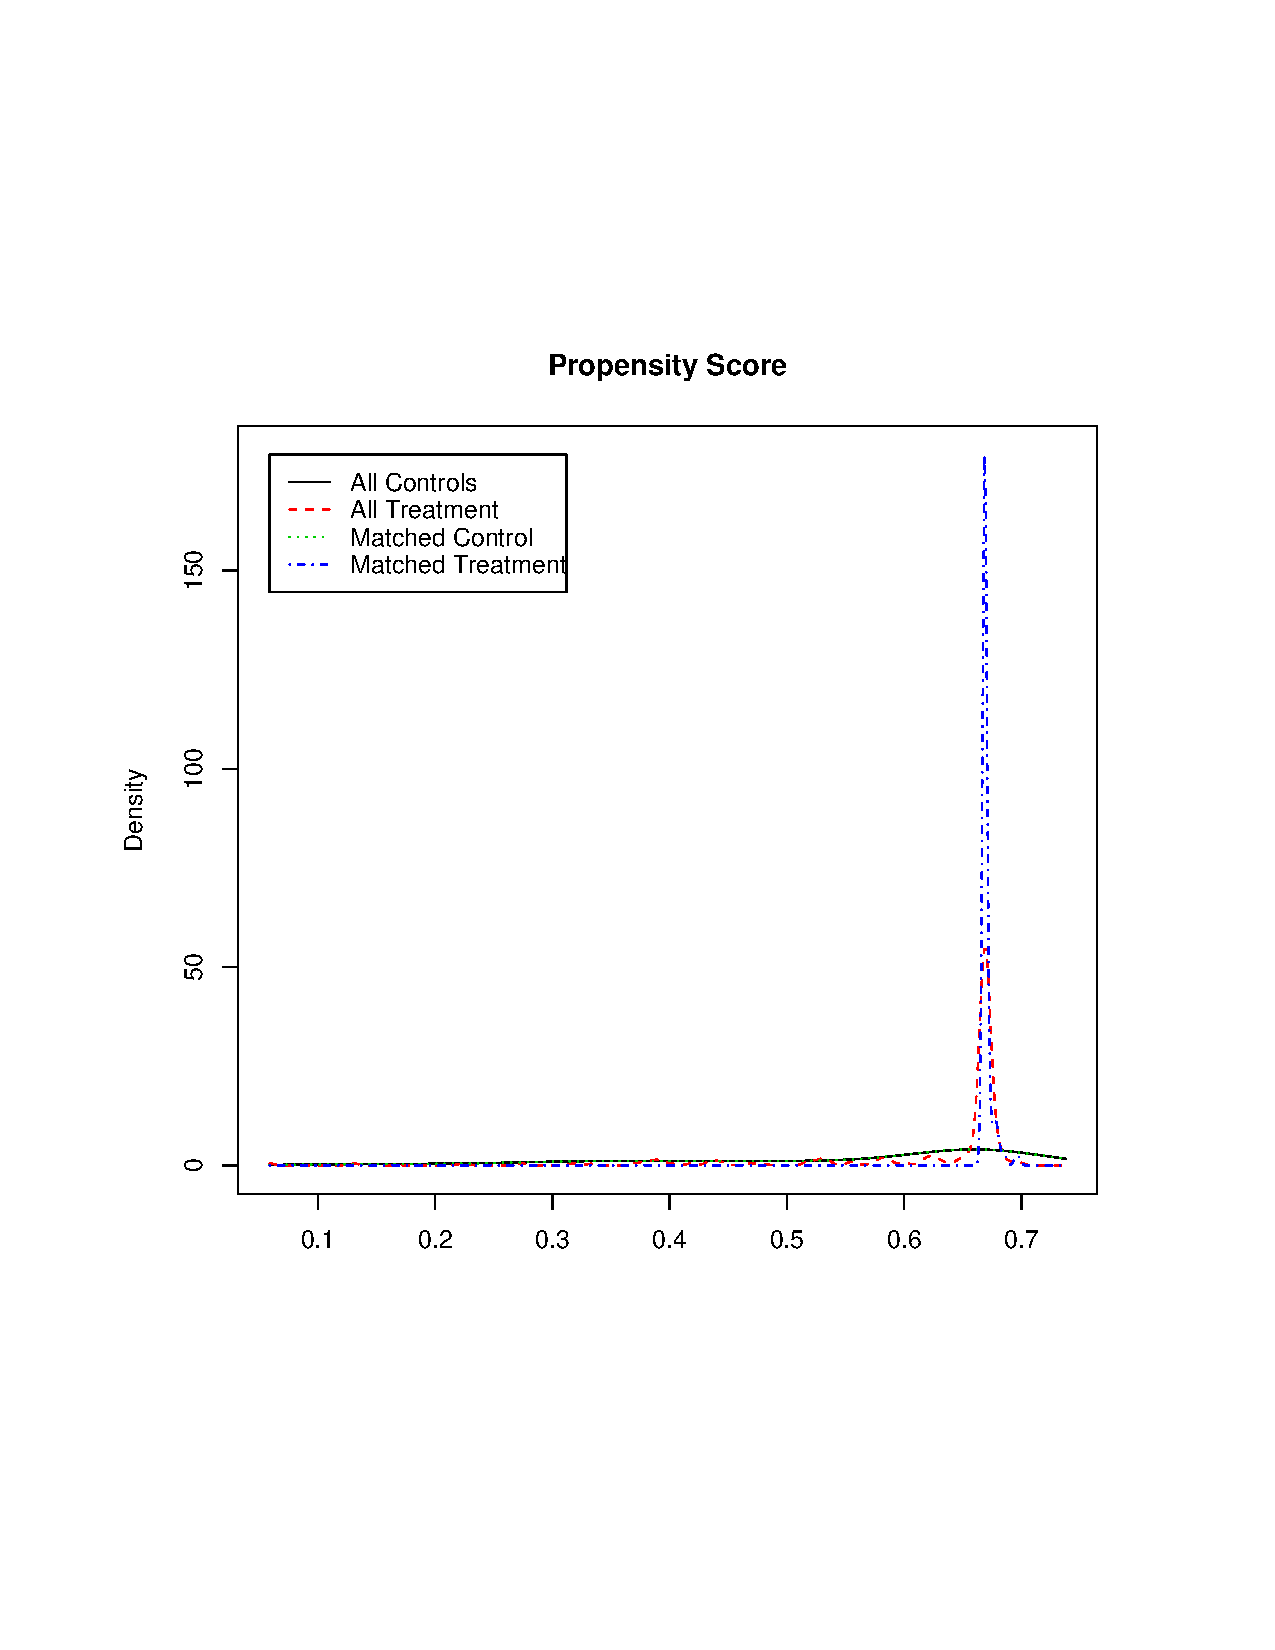
\includegraphics[width=2.35in,angle=0]{figs/f2pscore}
    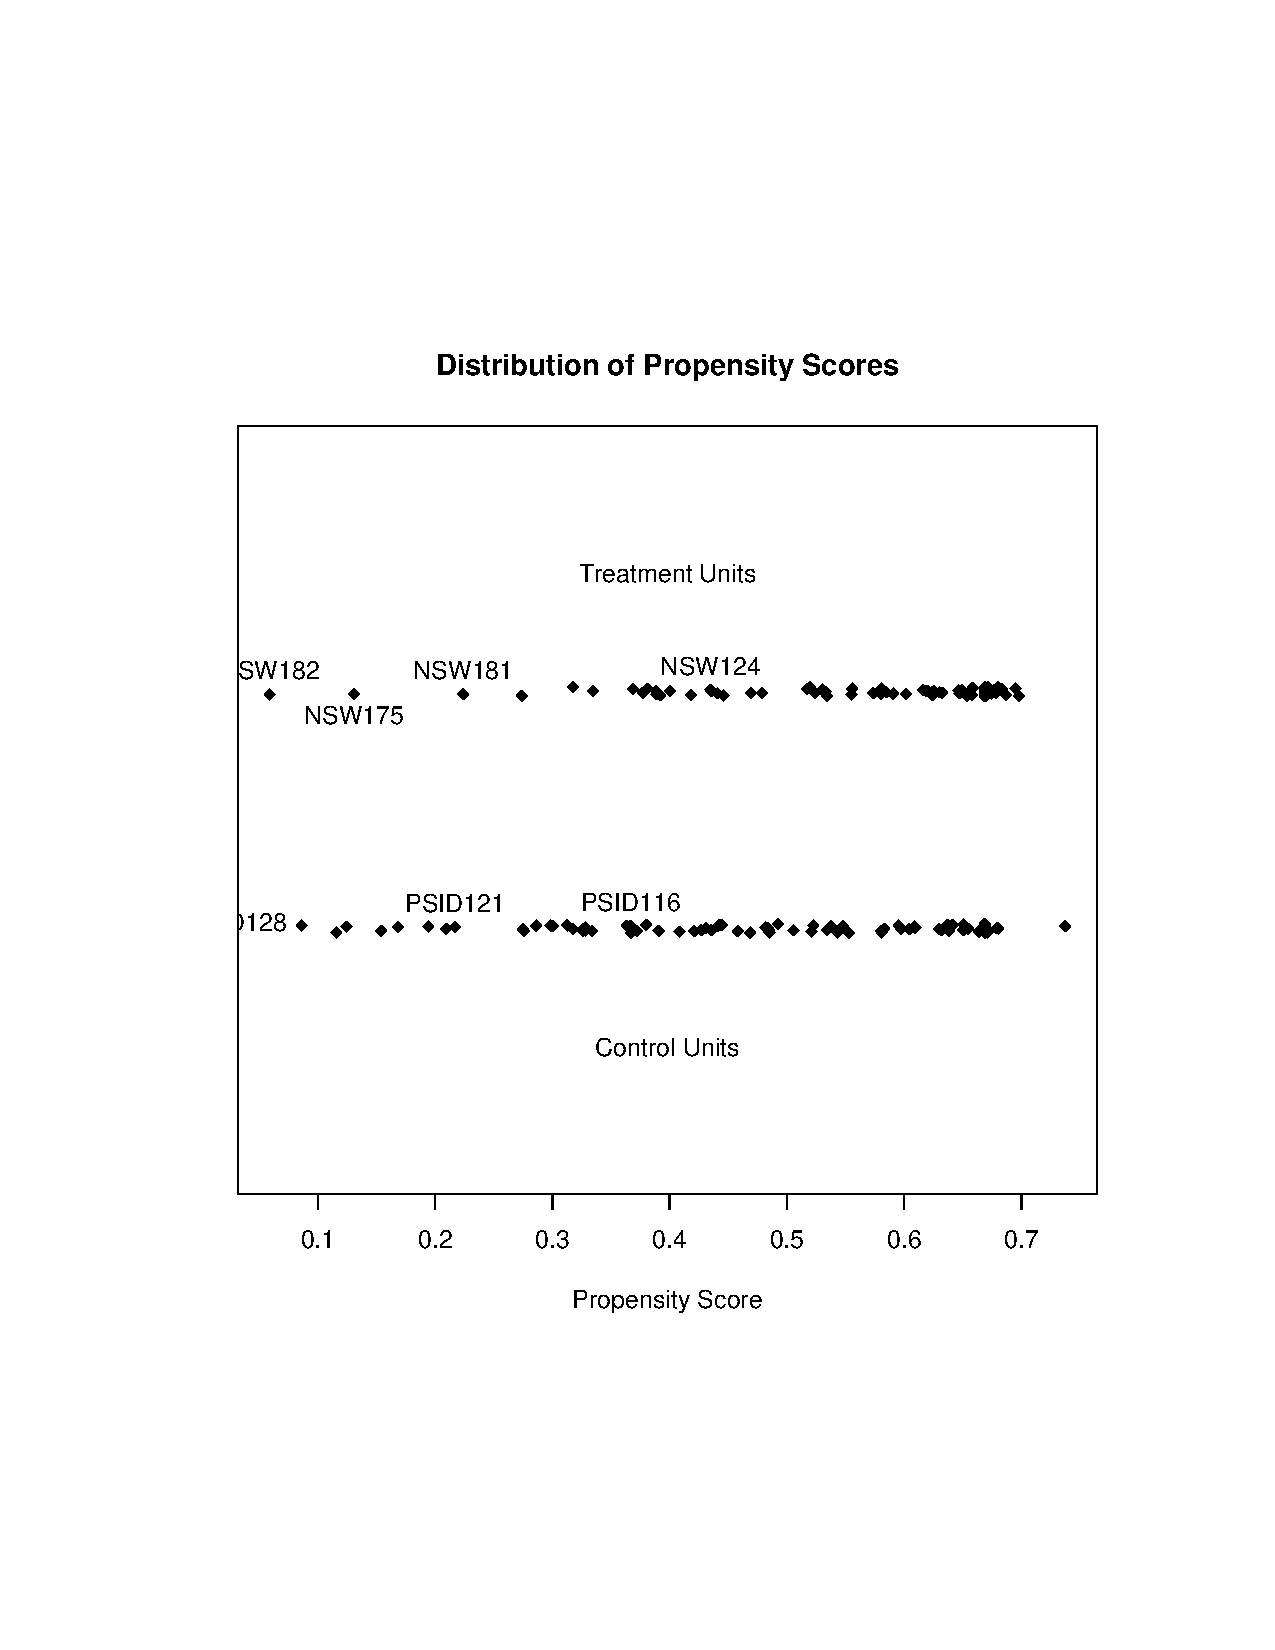
\includegraphics[width=2.35in,angle=0]{figs/f2pjitter}
    \hfill
    \caption{Sample interactive diagnostic graphs}
    \label{f2diags}
  \end{center}
\end{figure}

Examining these graphs in Figure~\ref{f2diags}, it does not appear from the left-hand graph (the first graph from the
\texttt{plot} command) that the matched samples
are quite similar.  In fact, as we noted before, the number of control units in the PSID sample is actually
less than the number of treated units.  This means that matching
without replacement is unlikely to decrease bias, since one is still
using all control units.  Hence, suppose we wanted to match with replacement:

\begin{verbatim}
> foo2a <- matchit(treat ~ re74 + re75, data=lalonde, replace=TRUE)
\end{verbatim} 

The diagnostic graphs in Figure~\ref{f2diags_replace} look somewhat better. 

\begin{figure}[h]
  \begin{center}
    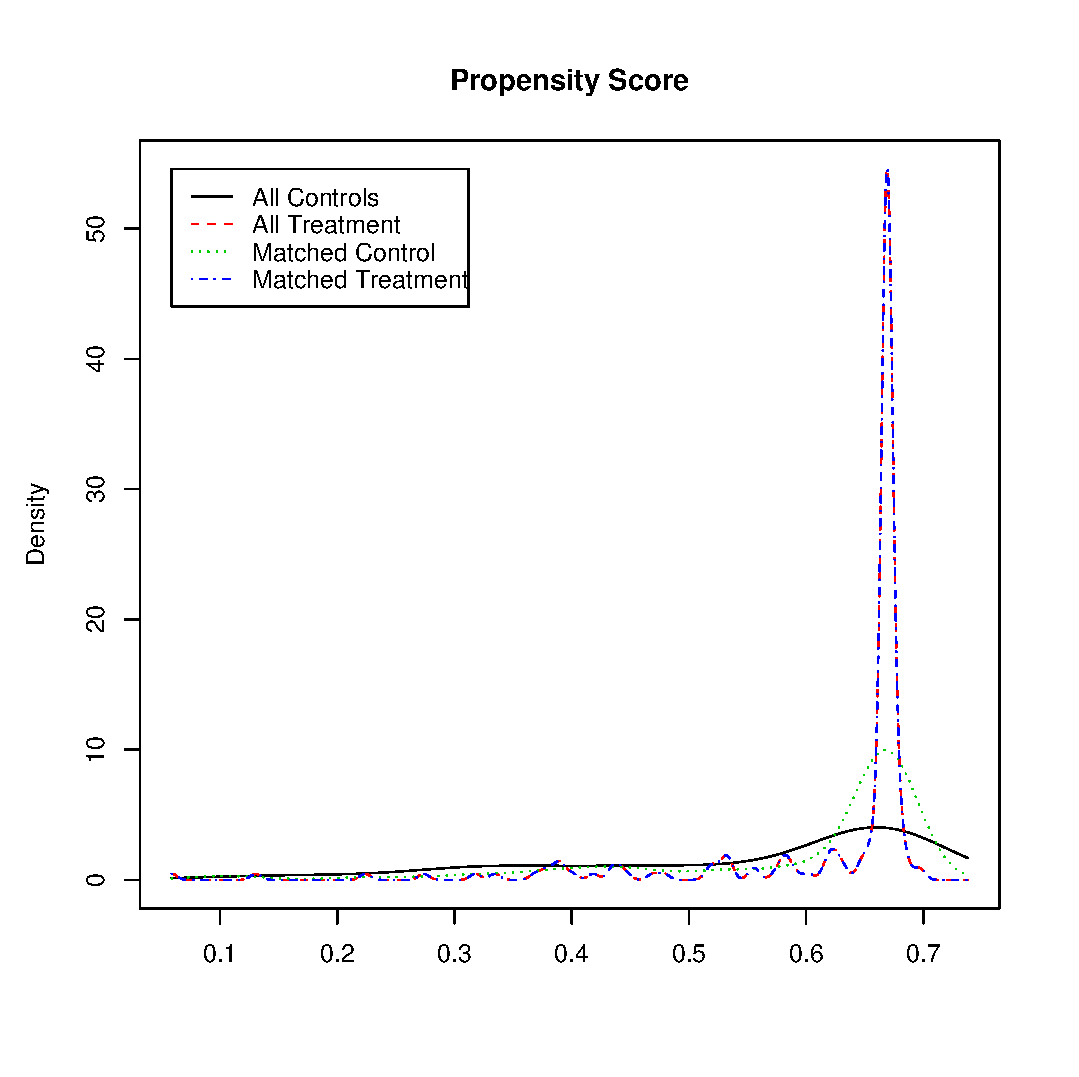
\includegraphics[width=2.35in,angle=0]{figs/f2pscore_r}
    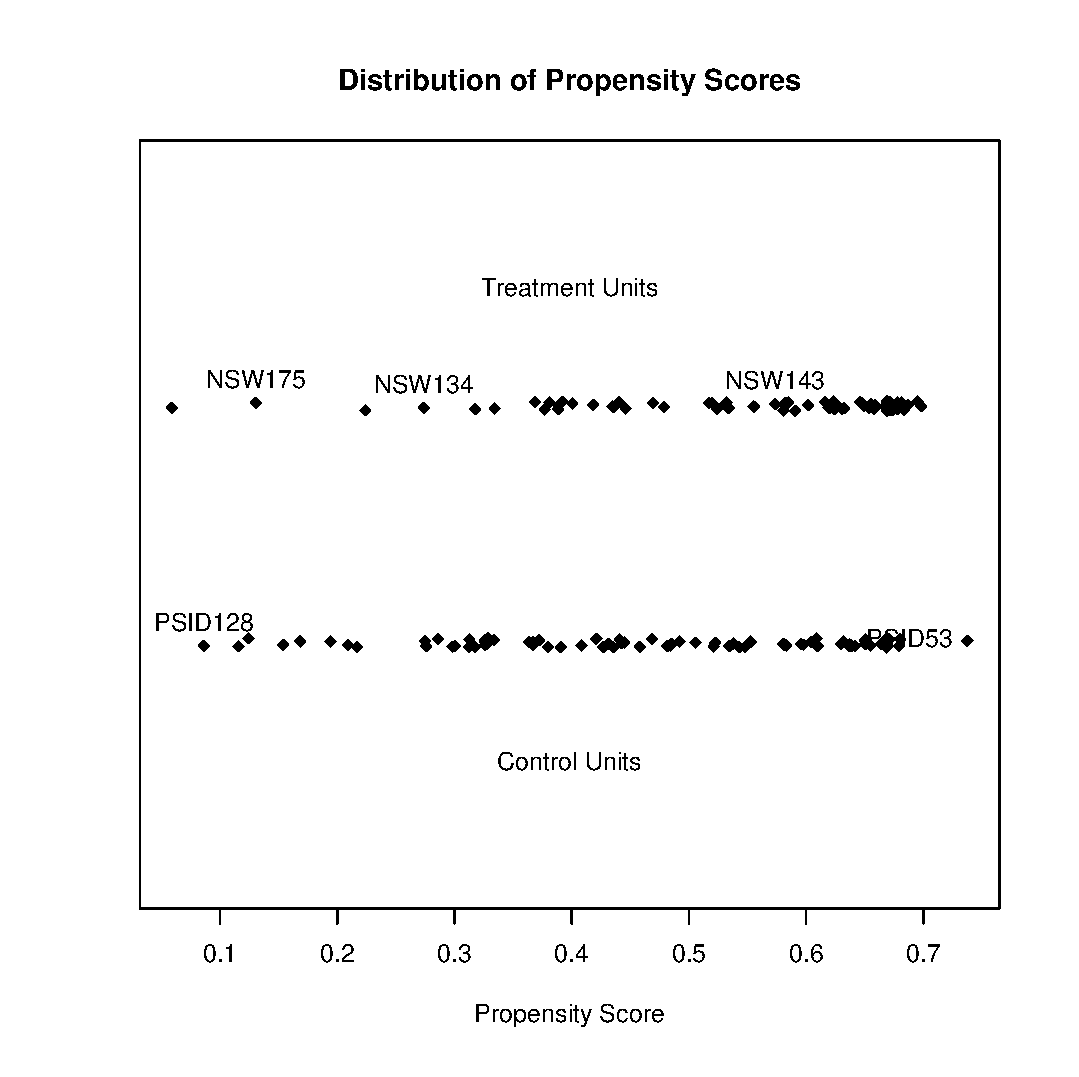
\includegraphics[width=2.35in,angle=0]{figs/f2pjitter_r}
    \hfill
    \caption{Sample interactive diagnostic graphs}
    \label{f2diags_replace}
  \end{center}
\end{figure}

We can also check means tests and balance statistics:

\begin{footnotesize}
\begin{verbatim}
> foo2a$sum.all
          means.t.all means.c.all       sd.all  t.all bias.all
pscore           0.62        0.54         0.14  -4.93     0.59
re74          2095.57     5566.87      6199.23   4.72    -0.56
re75          1532.06     2610.70      4362.80   1.97    -0.25
re74xre74 28141411.57 83216152.51 135805662.85   3.40    -0.41
re74xre75 13118578.32 31267090.48  72443160.98   1.98    -0.25
re75xre75 12654750.32 37625849.46  94943567.75   2.03    -0.26
Number         185.00      128.00       313.00 313.00   313.00
> foo2a$sum.matched
            means.t.m   means.c.m         sd.m t.matched bias.matched reduction
pscore           0.62        0.62         0.10     -1.85         0.00         1
re74          2095.57     2041.34      4775.26      1.71         0.01         1
re75          1532.06     1251.34      3071.87      0.21         0.06         1
re74xre74 28141411.57 25740726.49 104469102.06      1.28         0.02         1
re74xre75 13118578.32  8967690.87  45198031.40      0.63         0.06         1
re75xre75 12654750.32  9975368.67  53256124.72      0.60         0.03         1
Number         185.00       80.00       265.00    265.00       265.00       265
\end{verbatim}
\end{footnotesize}

which may also be obtained by using the \texttt{summary} command:

\begin{footnotesize}
\begin{verbatim}
> summary(foo2a)

Assignment model specification:
matchit(formula = treat ~ re74 + re75, data = lalonde, replace = TRUE)

Summary of covariates and interactions for all data:

          means.t.all means.c.all       sd.all  t.all bias.all
pscore           0.62        0.54         0.14  -4.93     0.59
re74          2095.57     5566.87      6199.23   4.72    -0.56
re75          1532.06     2610.70      4362.80   1.97    -0.25
re74xre74 28141411.57 83216152.51 135805662.85   3.40    -0.41
re74xre75 13118578.32 31267090.48  72443160.98   1.98    -0.25
re75xre75 12654750.32 37625849.46  94943567.75   2.03    -0.26
Number         185.00      128.00       313.00 313.00   313.00

Summary of covariates and interactions for matched data:

            means.t.m   means.c.m         sd.m t.matched bias.matched reduction
pscore           0.62        0.62         0.10     -1.97         0.00         1
re74          2095.57     2041.34      4775.68      1.84         0.01         1
re75          1532.06     1251.34      3072.15      0.32         0.06         1
re74xre74 28141411.57 25740726.49 104478317.35      1.36         0.02         1
re74xre75 13118578.32  8967690.87  45202018.35      0.70         0.06         1
re75xre75 12654750.32  9975368.67  53260822.48      0.66         0.03         1
Number         185.00       77.00       262.00    262.00       262.00       262

Problematic covariates:  
Number of units discarded:   0
\end{verbatim}
\end{footnotesize}

There are no longer substantially different 1974 or 1975 real earnings in the
matched sample, and the bias has substantially reduced in the
propensity score and real earnings.  More specifically, job training
participants on average earned roughly \$3,470 less in 1974 and \$1,080 less in 1975 than
non-participants, significant differences with t-statistics of
4.72 and 1.97, respectively.  In the matched sample, the earnings difference
is only \$54 (t-statistic=1.71) in 1974 and \$281 (t-statistic=0.21)
in 1975.  Note that \texttt{sum.all} and
\texttt{sum.matched} automatically calculate the statistics for all
squares and interactions of covariates specified in the assignment
model, which is helpful for diagnosing whether balance across
matched pairs has been attained.  Significant differences in higher
order interactions usually are a good indication that the assignment
model needs to be respecified.  The balance bias statistics,
calculated in the 
\texttt{reduction} column in \texttt{sum.matched}, additionally
indicate that there was an absolute
reduction in the balance bias in propensity scores and real earnings.

The \texttt{summary} command will additionally report (a) the original
call of the \MatchIt\ object, (b) whether there are any ``Problematic
covariates'' that may still be imbalanced in the assignment model, and
(c) how many units were discarded due to the \texttt{discard} option
(described below). 

Note also that only 80 control units were used in the matching
process, as seen the \texttt{Number} row of \texttt{sum.matched}. 
By looking at \texttt{foo2a\$weights} we can also examine how many times each of the control units was
matched to a treated unit.

\begin{footnotesize}
\begin{verbatim}
> foo2a$weights[foo2a$treat==0]
  PSID1   PSID2   PSID3   PSID4   PSID5   PSID6   PSID7   PSID8   PSID9  PSID10 
      2       1       3       2       0       2       1       2       2       2 
 PSID11  PSID12  PSID13  PSID14  PSID15  PSID16  PSID17  PSID18  PSID19  PSID20 
      2       0       1       2       4       4       5       3       1       1 
 PSID21  PSID22  PSID23  PSID24  PSID25  PSID26  PSID27  PSID28  PSID29  PSID30 
      4       1       1       3       2       4       1       4       3       3 
....
\end{verbatim}
\end{footnotesize}

\subsection{Propensity Score Matching with Exact Restriction}

Now suppose we wanted to match on a propensity score specification with only real earnings in 1974, 
as well as exact match on race:

\begin{verbatim}
> foo3 <- matchit(treat ~ re74, exact=c("black","hispan"),
  data=lalonde)
\end{verbatim}

We can easily verify that the race variables in the matched samples
are the same:

\begin{verbatim}
> foo3$sum.all[c("hispan","black"),]
       means.t.all means.c.all sd.all t.all bias.all
hispan        0.06        0.12   0.28  1.73    -0.21
black         0.84        0.45   0.47 -7.55     0.84
> foo3$sum.matched[c("hispan","black"),]
       means.t.m means.c.m sd.m t.matched bias.matched reduction
hispan      0.13      0.13 0.33         0            0         1
black       0.67      0.67 0.47         0            0         1
\end{verbatim}

Before matching, 84\% of participants were black, compared to only
45\% of the non-participants.  In the matched samples, black participants
and non-participants comprise 67\% of the observations. 

It is also easy to extract the matched subsetted data:
% ** [are we
% outputting this directly for Zelig portion -- currently even with
% weights, we can't... Why not? With the weights, can't we just
% output data[weights!=0,]?? That will output all of the people
% in data who were matched, and it works because weights should have the same
% length as the number of observations in data.  (liz) ]:

\begin{verbatim}
> fm <- na.omit(foo3$match.matrix)            #deleting non-matched units
> matched.treated <- lalonde[row.names(fm),]  #subsetting treated units
> matched.controls <- lalonde[as.character(fm[,1]),]        #subsetting control units
\end{verbatim}

We can further verify that every matched pair is identical
in \texttt{black} and \texttt{hispan}:

\begin{verbatim}
> mt <- matched.treated[,c("black","hispan")]  # subsetting the race indicators
> mc <- matched.controls[,c("black","hispan")]
> attributes(mt) <- NULL   # to strip names for identical() test
> attributes(mc) <- NULL
> identical(mt,mc)  #testing whether the arrays are identical
[1] TRUE
\end{verbatim}

\subsection{Replication of Dehejia \& Wahba}

The following line replicates the matching algorithm of Table 2
(column 10, row 4) of \citet{DehWah99}:

\begin{verbatim}
> data(lalonde)                 #calls the Lalonde data
> foo <- matchit(treat ~ age + I(age^2) + educ + I(educ^2) + black +
  hispan + married + nodegree + re74  + I(re74^2) + re75 + I(re75^2) +
  I(as.numeric(re74==0)) + I(as.numeric(re75==0)), data=lalonde,
  replace=1,discard=1)
\end{verbatim}

Note that the only differences between this and the earlier propensity
score matching example are: (a) the number of covariates used,  (b)
the \texttt{discard} option (which drops control units outside
the support of the treated group's propensity scores, and (c) matching with replacement. 

\subsection{Non-matched and Discarded Units}
The objects \texttt{in.sample} and \texttt{weights} give you all the
information about non-matched and discarded units.  \texttt{in.sample}
is a logical vector that indicates whether the unit was discarded due
to the common support conditions (the \texttt{discard} option), while
\texttt{weights} gives information on whether the unit was matched.
If for observation $i$, \texttt{in.sample}[i] is TRUE and
\texttt{weights}[i] is $0$, then unit $i$ was eligible for matching
but not used.  If \texttt{in.sample}[i] is FALSE, then
\texttt{weights}[i] will be $0$.  

For example, suppose we run the following assignment model:

\begin{verbatim}
> foo <- matchit(treat ~ age + educ, data=lalonde, discard=2, replace=TRUE)
\end{verbatim}

We can tell which units were discarded because of support conditions:

\begin{verbatim}
> foo$in.sample[!foo$in.sample]
  PSID4  PSID10  PSID12  PSID13  PSID22  PSID24  PSID27  PSID29  PSID30  PSID33 
  FALSE   FALSE   FALSE   FALSE   FALSE   FALSE   FALSE   FALSE   FALSE   FALSE 
 PSID37  PSID38  PSID48  PSID56  PSID79  PSID87 PSID103 PSID109 PSID110 PSID115 
  FALSE   FALSE   FALSE   FALSE   FALSE   FALSE   FALSE   FALSE   FALSE   FALSE 
PSID116 PSID127 
  FALSE   FALSE 
\end{verbatim}

And we can also tell which units were not matched despite meeting
support conditions:

\begin{verbatim}
> foo$weights[foo$in.sample & foo$weights==0]
  PSID1   PSID3   PSID5   PSID6   PSID7   PSID8   PSID9  PSID11  PSID15  PSID16 
      0       0       0       0       0       0       0       0       0       0 
 PSID17  PSID19  PSID20  PSID23  PSID28  PSID32  PSID35  PSID36  PSID39  PSID41 
      0       0       0       0       0       0       0       0       0       0 
 PSID42  PSID44  PSID45  PSID46  PSID49  PSID51  PSID52  PSID55  PSID57  PSID59 
      0       0       0       0       0       0       0       0       0       0 
 PSID70  PSID81  PSID84  PSID85  PSID91  PSID94  PSID95  PSID99 PSID100 PSID101 
      0       0       0       0       0       0       0       0       0       0 
PSID104 PSID106 PSID108 PSID112 PSID117 PSID118 PSID120 PSID124 
      0       0       0       0       0       0       0       0 
\end{verbatim}

One could further wonder how the discarded units differ from the
treated units in the NSW experiment:

\begin{verbatim}
> sdisc <- apply(lalonde[!foo$in.sample,],2,mean)   #taking column-wise means
> streat <- apply(lalonde[lalonde$treat==1,],2,mean)
> round(rbind(sdisc,streat),2)                      #rounding 
       treat   age  educ black hispan married nodegree    re74    re75    re78
sdisc      0 53.23 11.00  0.23   0.18    1.00     0.36 5027.30 2752.70 1054.56
streat     1 25.82 10.35  0.84   0.06    0.19     0.71 2095.57 1532.06 6349.14
\end{verbatim}

So the units that were discarded because of support conditions were on
average more than twice as old as the treated units, were much less
likely to be black, were all married, and much more likely to have
high school degrees.  

\subsection{Subclassification}

To perform a subclassification routine, use the \texttt{subclass}
command:

\begin{verbatim}
> data(lalonde) 
> foo1 <- matchit(treat ~ age + educ + black + hispan + married +
  nodegree + re74 + re75, data=lalonde, replace=TRUE, subclass=6)
\end{verbatim}

To perform subclassification on \emph{all} units, we can circumvent
the nearest neighbor matching algorithm entirely by setting
\texttt{nearest} to \texttt{FALSE}:

\begin{verbatim}
> data(lalonde) 
> foo2 <- matchit(treat ~ age + educ + black + hispan + married +
  nodegree + re74 + re75, data=lalonde, nearest=FALSE, replace=TRUE,
  subclass=6)
> print(foo2$match.matrix) %$
[1] NA
\end{verbatim}

Figure \ref{diags} presents diagnostic graphs from \texttt{plot(foo2)}.  

\begin{figure}[tbp]
  \begin{center}
    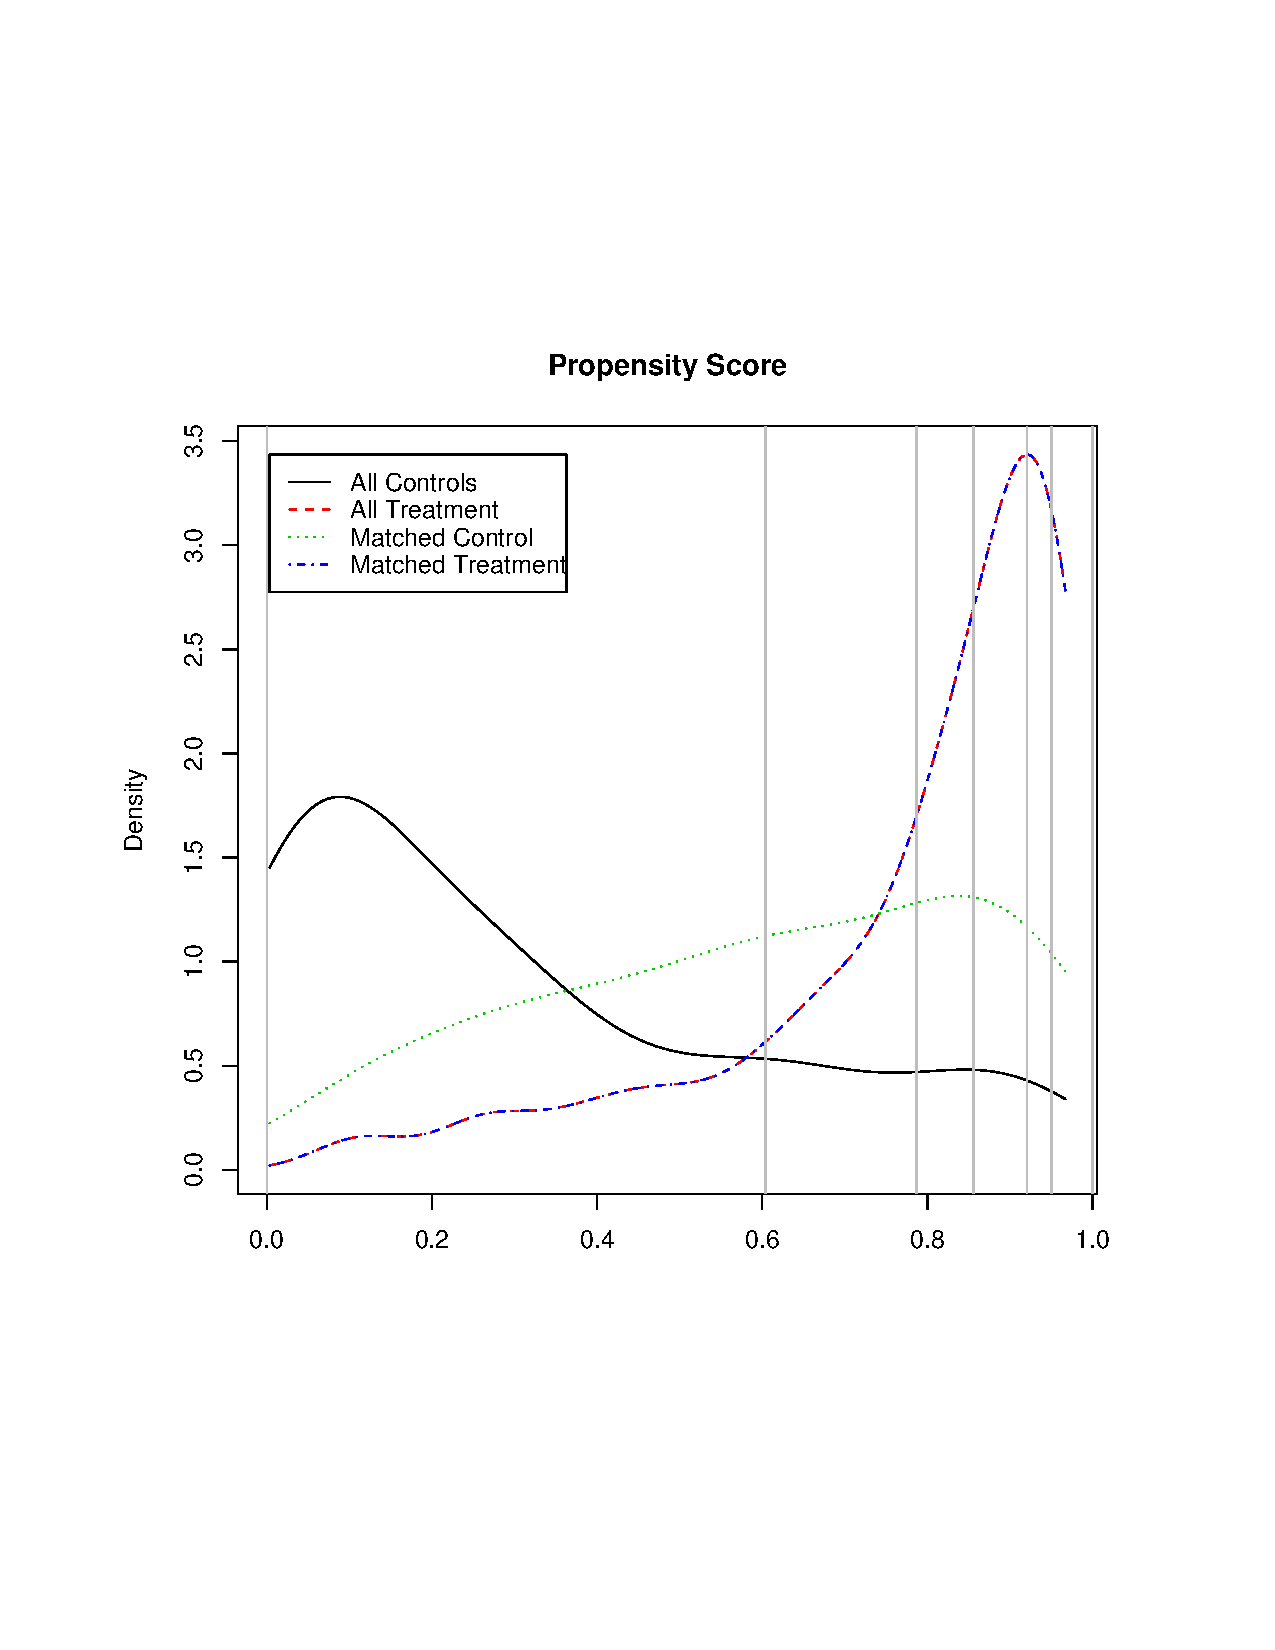
\includegraphics[width=2.35in,angle=0]{figs/pscore}
    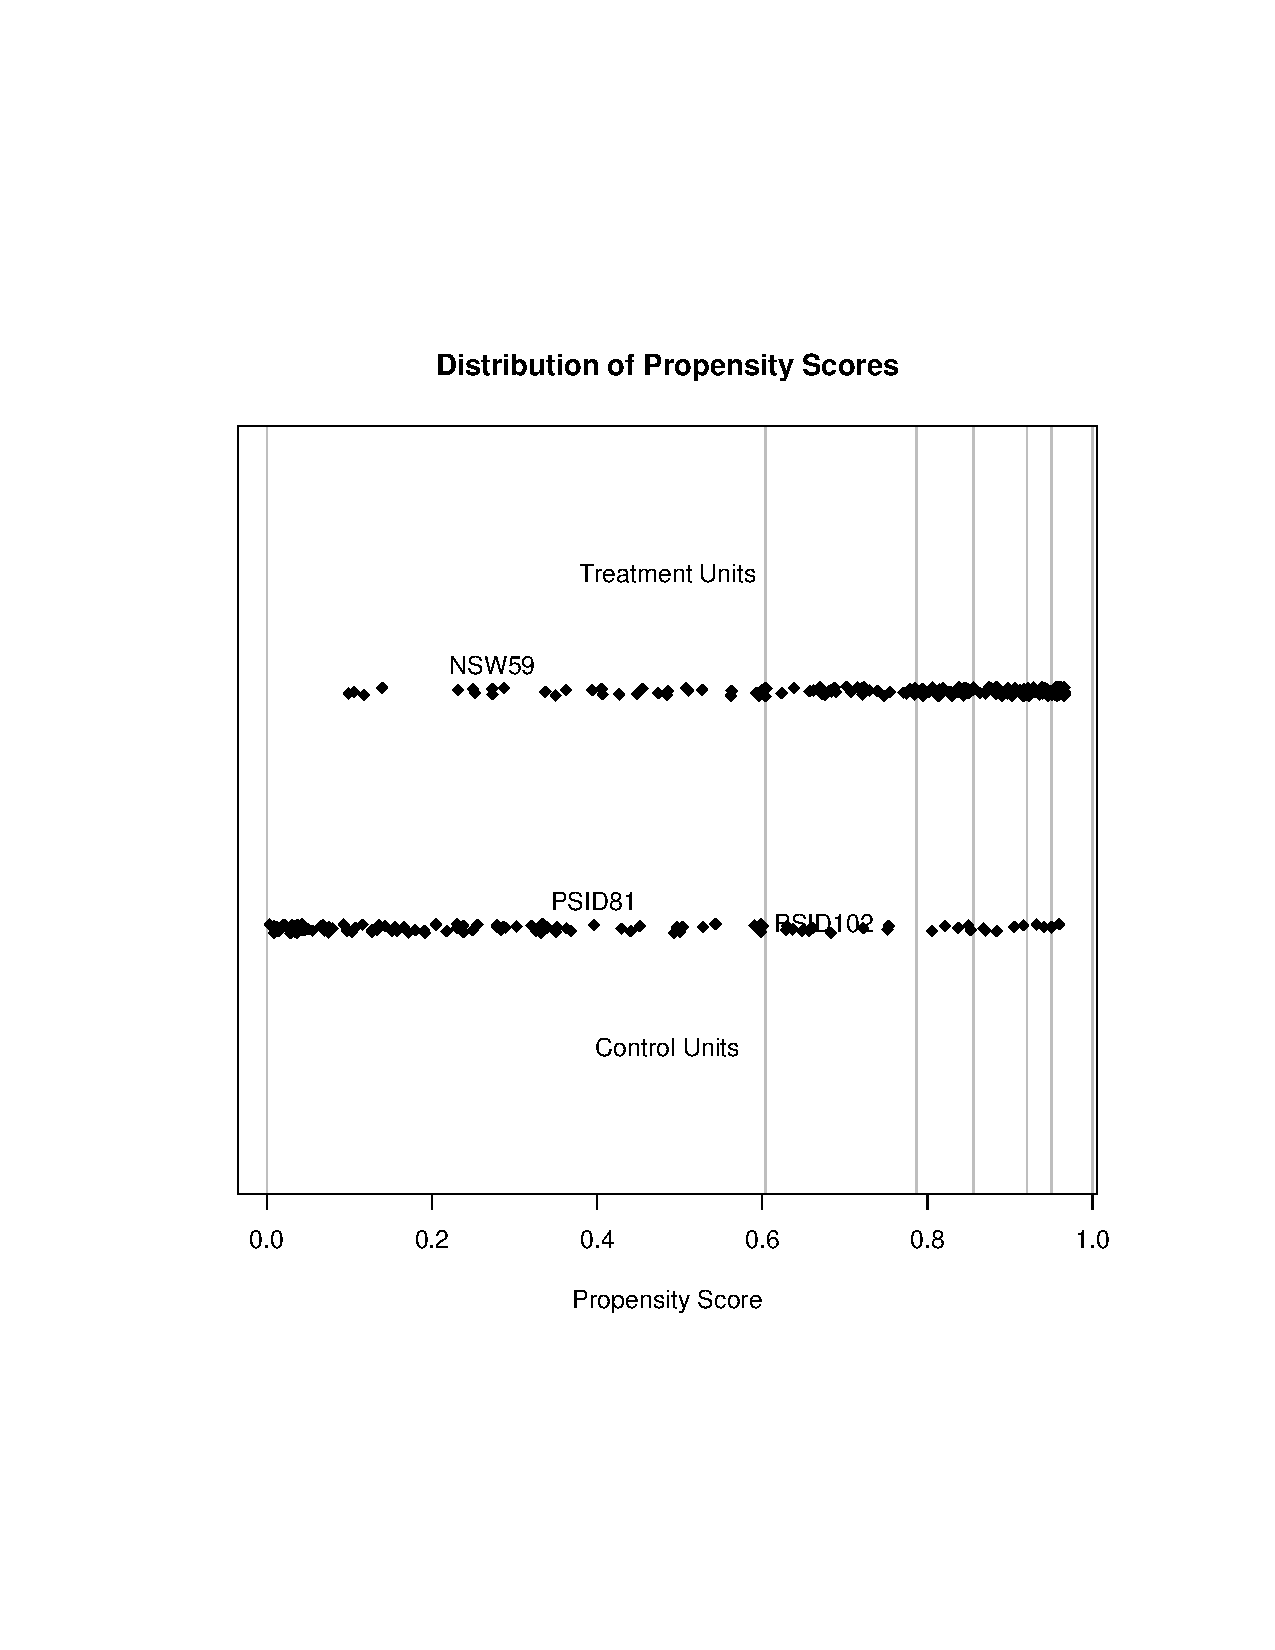
\includegraphics[width=2.35in,angle=0]{figs/pjitter}
    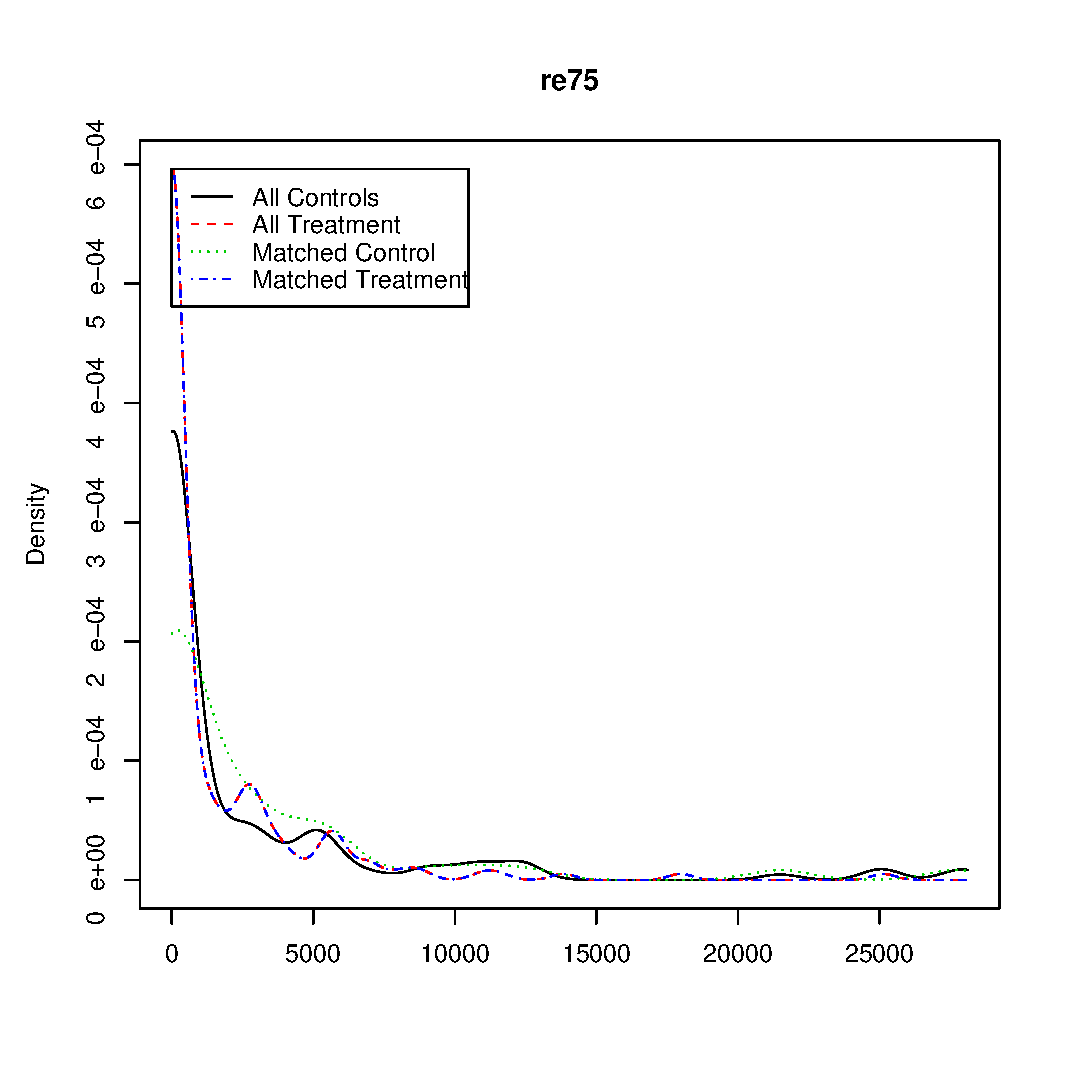
\includegraphics[width=2.35in,angle=0]{figs/re75dens}
    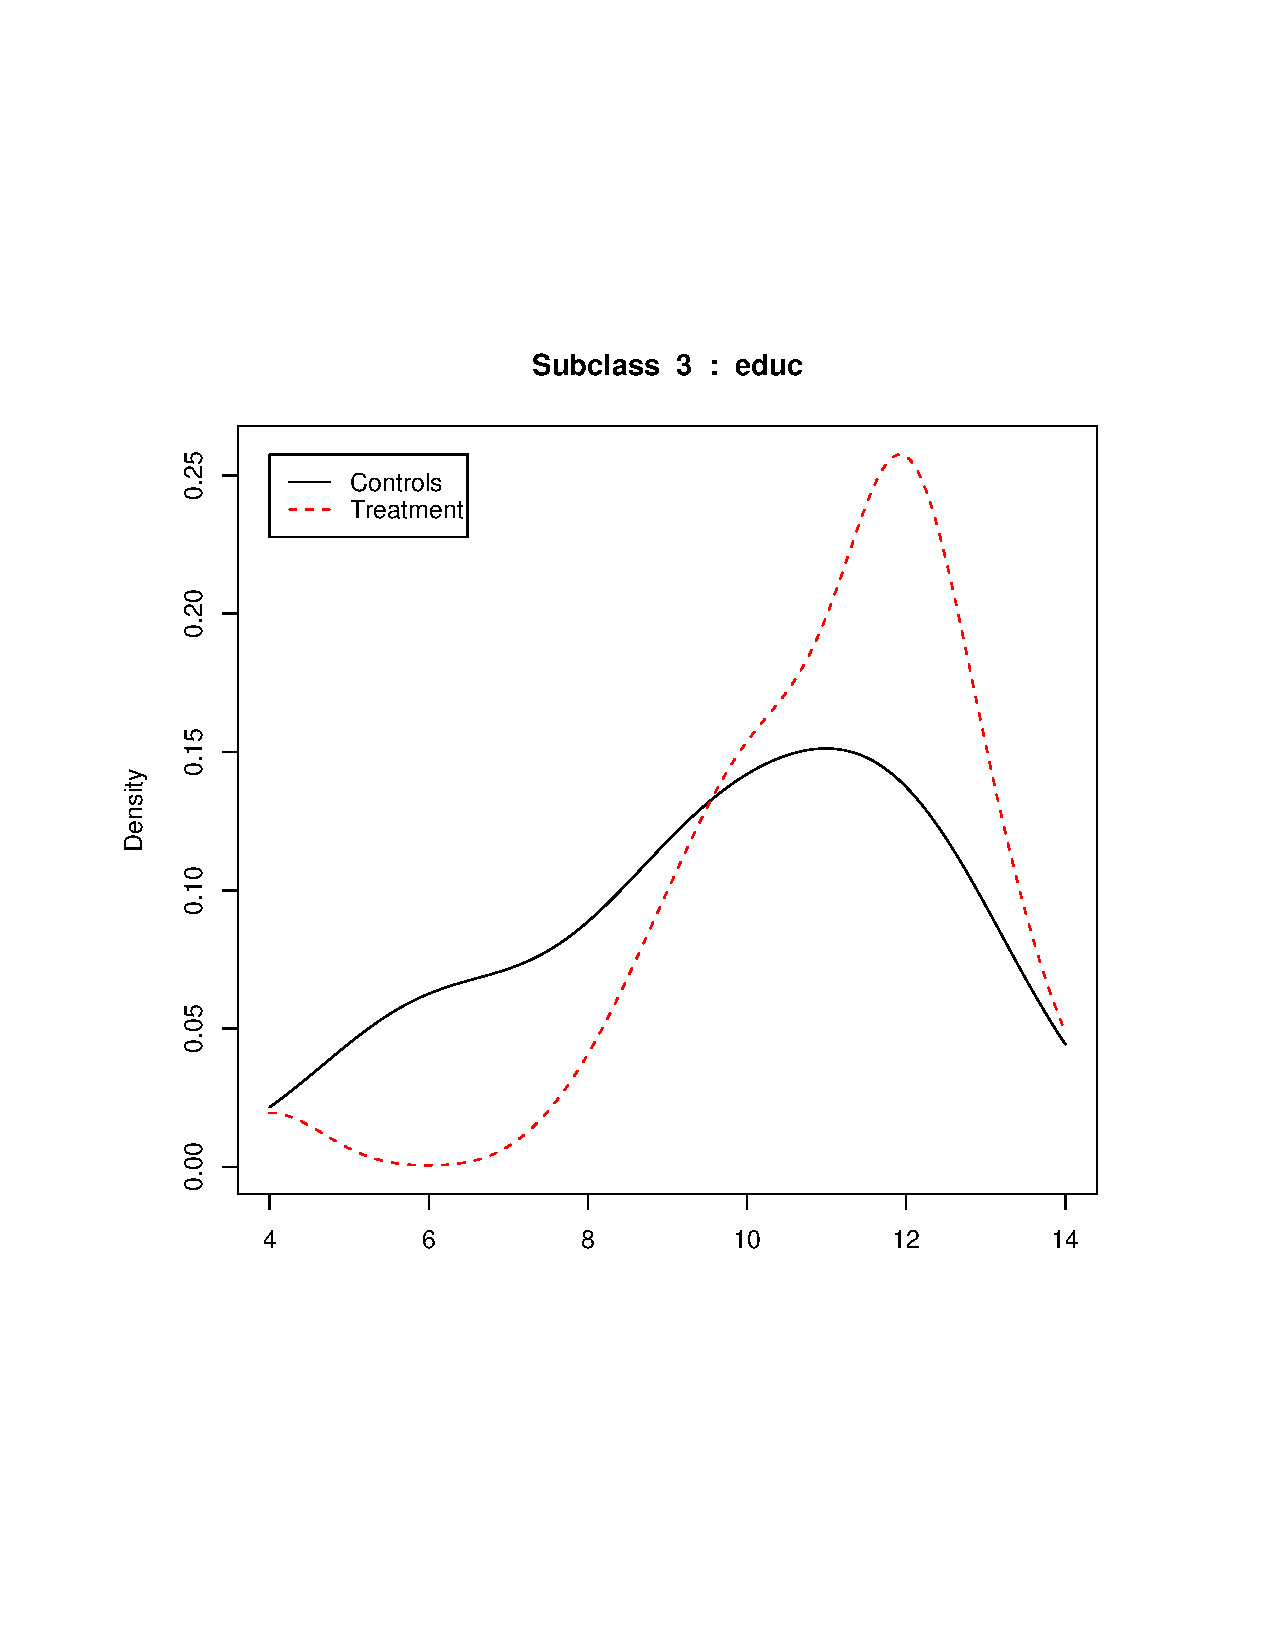
\includegraphics[width=2.35in,angle=0]{figs/sub3educ}
    \hfill
    \caption{Sample interactive diagnostic graphs from \texttt{demo(lalonde)}}
\label{diags}
\end{center}
\end{figure}

\texttt{q.table} can be an easy way to provide summaries across
subclasses.  For example, to examine summary statistics for the
propensity score across all six subclasses:

\begin{footnotesize}
\begin{verbatim}
> foo1$q.table[1,,]
            Subclass 1 Subclass 2 Subclass 3 Subclass 4 Subclass 5 Subclass 6
means.t.q         0.39       0.71       0.83       0.89       0.94       0.96
means.c.q         0.40       0.70       0.83       0.90       0.94       0.96
sd.q              0.16       0.05       0.02       0.02       0.01       0.00
t.q               0.31      -0.54       0.26       1.65       3.22      -0.10
bias.q           -0.04       0.02       0.00      -0.02      -0.02       0.00
reduction.q       1.00       1.00       1.00       1.00       1.00       1.00
\end{verbatim}
\end{footnotesize}

Or to examine for how many covariates, squares and interactions there's been a reduction in the
``balance bias'' for each subclass: 

\begin{footnotesize}
\begin{verbatim}
> apply(foo1$q.table[,6,]==1,2,sum,na.rm=T)
Subclass 1 Subclass 2 Subclass 3 Subclass 4 Subclass 5 Subclass 6 
        30         24         23         31         42         38 
\end{verbatim}
\end{footnotesize}

\subsection{Exact Matching on All Covariates}

To match exactly on all covariates:

\begin{verbatim}
> foo <- matchit(treat ~ age + educ + black + hispan + married +
  nodegree + re74 + re75, data=lalonde, exact=TRUE, replace=TRUE)
\end{verbatim}

Or more simply,

\begin{verbatim}
> foo <- matchit(treat~age,exact=names(lalonde)[2:9],
  data=lalonde,replace=TRUE)
> print(na.omit(foo$match.matrix)) %$
           V1
NSW7   PSID50
NSW21  PSID49
NSW27  PSID14
NSW35  PSID40
NSW50  PSID50
NSW54  PSID40
NSW74  PSID40
NSW81  PSID40
NSW93  PSID14
NSW103 PSID14
\end{verbatim}

Hence out of the 185 observations in the NSW sample, only 10 exact
matches exist when matching with replacement.

\subsection{Caliper Matching}

To match within a caliper of 0.25 standard deviations of the
propensity score, use the \texttt{caliper} input:

\begin{verbatim}
> foo <- matchit(treat ~ age + educ + black + hispan + married +
  nodegree + re74 + re75, data=lalonde, caliper=0.25, replace=TRUE)
\end{verbatim}

This restricts the matches to have propensity scores within the
caliper size.  It is usually used in combination with Mahalanobis
matching, as described in Section \ref{mahal}.

If no control units exist within the range of caliper specified, the
treated unit remains unmatched.  In some instances this might result
in very few matched units.  As a result, you may want to increase the
caliper size or match nearest neighbors when no units within the
caliper are available by specifying \texttt{calclosest=TRUE}.

\subsection{Mahalanobis Metric Matching within Caliper}
\label{mahal}
To match with the Mahalanobis metric within the caliper, specify the
variables on which to compute the metric with the \texttt{mahvars}
input, and the \texttt{caliper} input:

\begin{verbatim}
> foo <- matchit(treat ~ age + educ + black + hispan + married +
  nodegree + re74 + re75, data=lalonde, mahvars=c("age","educ"),
  caliper=0.25, replace=TRUE)
\end{verbatim}

\subsection{Mahalanobis Metric Matching}

To perform only Mahalanobis Metric matching, set the
\texttt{caliper=Inf}:

\begin{verbatim}
> foo <- matchit(treat ~ age + educ, data=lalonde,
  mahvars=c("age","educ"), caliper=Inf, replace=TRUE)
\end{verbatim}

\subsection{Assignment Model Specification}

\MatchIt\ permits you to use a wide variety of methods to
estimate the propensity score, including logit (default), probit,
neural networks, generalized additive models, and classification
trees.  These can be specified in the \MatchIt\ call using the
\texttt{model} input.  For example:

\begin{verbatim}
foo1 <- matchit(treat~educ+re74+re75,data=lalonde,model="probit")
foo2 <- matchit(treat~educ+re74+re75,data=lalonde,model="nnet")
foo3 <- matchit(treat~educ+re74+re75,data=lalonde,model="gam")
foo4 <- matchit(treat~educ+re74+re75,data=lalonde,model="cart")
\end{verbatim}

Each use different models to estimate the propensity score.  Before
using any of these techniques, the user is strongly advised to
seek outside resources to understand the theoretical groundings of
these techniques.  For political science articles discussing or
implementing (a) neural networks see
\citet{beck99,Zeng99,Zeng00,LagRus02}, (b) generalized
additive models see \citet{BecJac98}, and (c) classification trees
see \citet{RugKimMar03}.  For more general treatments,
see \citet{Bishop95,White92,BreFriOls84}. 
See also the \texttt{glm} library for further control of logit and
probit regressions, the \texttt{nnet} for neural networks, the
\texttt{mgcv} library for generalized additive models, and the
\texttt{rpart} library for classification trees.

\subsection{Using Observation Names}
\label{rnames}

Since the diagnostics often make use of the observation names of the
data frame, you may find it helpful to specify observation names the
data input.  Use the \texttt{row.names} command to achieve this.  For
example, to assign the names ``Dan'', ``Kosuke'', ``Liz'' and ``Gary''
to a data frame with the first four observations in the Lalonde data,
type: 

\begin{verbatim}
> test <- lalonde[1:4,]  #taking a lalonde subset
> row.names(test) <- c("Dan","Kosuke","Liz","Gary")  #assigning row names
> print(test)
       treat age educ black hispan married nodegree re74 re75      re78
Dan        1  37   11     1      0       1        1    0    0  9930.046
Kosuke     1  22    9     0      1       0        1    0    0  3595.894
Liz        1  30   12     1      0       0        0    0    0 24909.450
Gary       1  27   11     1      0       0        1    0    0  7506.146
\end{verbatim} 

\subsection{Matching on One Covariate}
\MatchIt\ does not assume a propensity score bounded between 0 and 1.
For example, we could use simply the \texttt{matchdef} command,
documented in Appendix~\ref{reference}, to match nearest neighbors on
one covariate:

\begin{verbatim}
index <- rep(TRUE,nrow(lalonde))   #keeping all units
names(index) <- row.names(lalonde) #assigning obs names
treat <- lalonde$treat
names(treat) <- row.names(lalonde)
re75 <- lalonde$re75
names(re75) <- row.names(lalonde)
foo <- matchdef(treat,index,re75,replace=TRUE)
\end{verbatim}

\section{Reference}

\subsection{Usage}

The basic syntax to \texttt{matchit} is quite similar to other models in R, such as the
\texttt{lm} or \texttt{glm} models: 

\begin{verbatim}
matchit <- function(formula, data=NULL, discard=0, exact=FALSE,
           replace=FALSE, ratio=1, model="logit", reestimate=FALSE,
           nearest=TRUE, m.order=2, caliper=0, calclosest=FALSE,
           mahvars=NULL, subclass=0, subtype=1, interact=TRUE, ...)
\end{verbatim}

\subsection{Inputs}

\begin{enumerate}

\item \textbf{Formula (required).}  \texttt{formula}  takes the form of {\tt T \~\ X1 + X2}, where
  {\tt T} is a binary treatment indicator and {\tt X1} and {\tt X2} are
  the pre-treatment covariates, and {\tt T}, {\tt X1}, and {\tt X2}
  are contained in the same data frame.  The $+$ symbol means
  ``inclusion'' not ``addition.'' You may also include
  interaction terms in the form of {\tt I(X1*X2)} or squared terms in
  the form of {\tt I(X1 \^\ 2)}.\footnote{The \texttt{I()} command
  ensures that the expression is interpreted as one term.  If you omit
  it, the main effects will automatically be included as well.} 
  
\item \textbf{Dataframe (required).}  \texttt{data} specifies the data frame containing the
  variables called in the formula.  You may find it helpful for the
  diagnostics to specify observation names in the data frame.  To do
  this, see Section~\ref{rnames}.

\item \textbf{Discarding.} \texttt{discard} specifies whether to discard units that
  fall outside some measure of support of the distance score
  \begin{itemize}
  \item default=0 keeps all units.  Use this
    option when the units to be matched are substantially similar,
    such as in the case of matching treatment and control units from a
    field experiment that was close to (but not fully) randomized
    (e.g., \citealt{Imai03}).  (Other reasons for
    keeping all units may be that subclassification on all units is
    desired or that caliper matching will naturally restrict the donor
    pool.)
  \item  1 keeps all units with common support on the distance
    measure. Use this option when the units to be
    matched are substantially different (i.e., when there is a large
    degree of non-overlapping support on the distance score), such as
    in the case of measuring the effect of democracy on economic
    growth (e.g., \citealt{KinZen03}).  
  \item 2 discards only control units outside the support of the
    distance measure of the treated units.
    Use this option when the average treatment effect on the treated
    is of most interest and when unwilling to discard non-overlapping
    treatment units, such as possibly in the case of the effect of job
    training on those individuals that actually participated in a job
    evaluation program (e.g., \citealt{HecIchTod98}) or a drug study
    where one cannot discard patients treated with the drug for
    whatever reason. 
  \item 3 discards only treated units outside the support of 
    the distance measure of the control units.  Use this option when
    the average treatment effect on the control units is of most
    interest and when unwilling to discard control units. 
  \end{itemize}

\item \textbf{Exact Matching.}  \texttt{exact} specifies whether exact
  matching should be done.  \texttt{FALSE} (default) indicates no exact 
  matching.  \texttt{TRUE} indicates exact matching on all variables in the 
  assignment model of the \texttt{formula} (i.e., the propensity score
  will never be generated).  A vector of variable names indicates separate variables on
  which to exact match, in combination with matching on the propensity
  score.  This option will not be different from \texttt{exact=TRUE},
  unless the list differs from the variables in the formula.\footnote{For
    example, \texttt{matchit(T \~\ X1 + X2, data, exact=TRUE)} is
    equivalent to \texttt{matchit(T \~\ X1, data, exact=cbind(X1,X2))}.
    But \texttt{matchit(T \~\ X1 + X2, data, exact=X1)} will match
    units exactly only on \texttt{X1} and perform nearest neighbor
    matching on the propensity score which uses \texttt{X1} and \texttt{X2}.} 
  Variables should be entered as a vector of names 
  \texttt{exact=c("X1","X2")} that refer to variable names in \texttt{data}.
  
\item \textbf{Replacement matching.} \texttt{replace} is a logical vector which specifies whether
  to match with replacement, default=FALSE.  Use this to reduce bias
  when the ratio of control units that are comparable to the treated units
  is small and when pre-treatment covariates between treatment and
  control units diverge substantially.  

\item \textbf{Ratio Matching.}  \texttt{ratio} specifies the number of
  control units to be matched to each treatment unit, default=1.  Use
  larger integer values when a large number of comparable control units are available to
  increase efficiency of the estimand. If matching is done without replacement and there are 
  fewer control units than ratio times the number of eligible treated units (i.e. not enough control
  units for the specified method), then the higher
  ratios will have \texttt{NA} in place of the matching unit number.  

\item \textbf{Assignment Model.}The assignment model estimation may be
  changed by \texttt{model}, which specifies the method used to estimate the propensity score:
  \begin{enumerate}
  \item \texttt{logit}, the default method, implements a logistic regression.  See
    {\tt help(glm)} for more options. 
  \item \texttt{probit} implements a probit regression.  See
    {\tt help(glm)} for more options. 
  \item \texttt{nnet} implements a neural network in the
    \texttt{nnet} library, with a default size of 3.  See {\tt
      help(nnet)} for more options.
  \item \texttt{GAM} implements a generalized additive model 
    as in the \texttt{mgcv} library.  See
    {\tt help(gam)} for more options.
  \item \texttt{cart} implements a classification tree as in the
    \texttt{rpart} library.  See {\tt help(rpart)} for more
    options.  
  \end{enumerate}

\item \textbf{Reestimation.} \texttt{reestimate} specifies whether the
  propensity score model should be re-estimated after units are
  discarded, default=FALSE.  This may be desirable for efficiency
  reasons. 
% ** [but we have no formal proof for this, right?].  
  
\item \textbf{Advanced Matching}
  \begin{itemize}
  \item \texttt{nearest} is a logical scalar which specifies whether
    to perform nearest-neighbor matching, default=TRUE.  If
    \texttt{nearest=FALSE} this can provide a more efficient way to
    perform only subclassification. 
  \item \texttt{m.order}  specifies the order within which to match
    treatment units with control units
    \begin{itemize}
    \item (2) indicates matching from highest propensity scores to
      lowest (default)
    \item (3) indicates matching from lowest propensity scores to
      highest
    \item (4) indicates matching in random order
    \item (1) is a placeholder for optimal matching that is yet to be
      developed 
    \end{itemize}
  \item \texttt{caliper} specifies the standard deviations of 
    the propensity score within which to draw control units,
    default=0.  If \texttt{caliper!=0}: 
    \begin{itemize} 
    \item \texttt{calclosest} specifies whether to take nearest
      available match if no matches are available within
      \texttt{caliper}, default=FALSE 
    \item \texttt{mahvars} specifies
      variables on which to perform Mahalanobis-metric matching
      within each caliper, default=NULL.  Variables should be entered
      either as a vector of variable names
      \texttt{mahvars=c("X1","X2")} that are names of variables in
      \texttt{data}. 
    \end{itemize}
  \end{itemize}

\item \textbf{Subclassification}
  Subclassification options allow the user to subclassify units along
  the propensity score:
  \begin{itemize}
  \item \texttt{subclass} is either (1) a scalar, specifying the number of
    subclasses, or (2) a vector of probabilities bounded
    between 0 and 1, to create quantiles based on \texttt{subtype}, where the value of
    0 (default) indicates no subclassification.  
  \item If \texttt{subclass!=0}, \texttt{subtype} may specify by what
    criteria to subclassify: (0) indicates by the number of control
    units, (1) indicates by number of treatment units (default), and
    (2) indicates by the total number of units.  
  \end{itemize}
  The subclass options create quantiles corresponding to the given
  probabilities from \texttt{subclass}, using the \texttt{quantile}
  command on the propensity scores of the \texttt{subtype} units. 
\end{enumerate}
  
\subsection{Output}

The following are the outputs of each \texttt{matchit} object, though
note that if outputs are not applicable for the original
\texttt{matchit} call, they will be returned as \texttt{NA}): 

\begin{enumerate}
  
\item \texttt{match.matrix} is an $n_1$ by \texttt{ratio} data frame,
  where:
%** [Need to change match.matrix to match.frame]

  \begin{itemize}
  \item the row names, \texttt{row.names(match.matrix)}, store the
    names of the treatment units, which come from the data frame
    specified in \texttt{data} (to learn how to do this, see
    Section~\ref{rnames}),
  \item each column stores the name(s) of the control unit(s) matched
    to the treatment unit of that row (e.g., when the \texttt{ratio}
    input is specified as 3, the three columns of
    \texttt{match.matrix} represent the three control units matched to
    one treatment unit),
   \item \texttt{NA} indicates that the treatment unit was not
     matched.  
   \end{itemize}

See the simple example is Section~\ref{exactm} for an illustration of the
\texttt{match.matrix} format. 

\item \texttt{pscore} is a vector of $n$ length that contains the estimated propensity scores for
  all units (i.e., the probability of treatment assignment
  conditional on the covariates).

\item \texttt{in.sample} is a vector of $n$ length that
  displays whether the units were eligible for matching due to
  discarding.  If unit $i$ was discarded, \texttt{in.sample[i]=FALSE},
  and if unit $i$ was not discarded \texttt{in.sample[i]=TRUE}.

\item \texttt{weights} is a vector for all observations that provides
  the weights assigned to each unit in the 
  matching process.  Unmatched units have weights equal to $0$. Matched
  treated units have weight $1$.  Matched control units have weight $
  \sum_{i=1}^{N_m} \frac{1}{c_i} $, where the sum is over the treated
  units that control unit was matched
  to, and $c_i$ is the number of control units treated unit $i$
  was matched to.  The sum of the weights for the control group will equal 
  the number of treated units that were matched.  

\item \texttt{sum.all} is a data frame which contains variable names
  and interactions down the row names, and summary statistics on \emph{all
  observations} in each of the
  columns.  The columns in \texttt{sum.all} contain:
  \begin{itemize}
  \item means for treatment units of all covariates $X$ and their
    interactions, where \texttt{means.t.all}$= \mu_{X|T=1} =
    \frac{1}{n_1} \sum_{T=1} X_i$ and
    \texttt{means.c.all}$= \mu_{X|T=0} = \frac{1}{n_0} \sum_{T=0} X_i$,
  \item standard deviations for all covariates $X$ and their
    interactions, where \texttt{sd.all}$= s_X = \frac{1}{n-1}
    \sum_{i} (X_i - \overline{X})$,
  \item t-statistics from means tests of all covariates $X$ and their
    interactions \texttt{t.all},\footnote{Note that the t-tests do
      not assume constant variance across treatment and control
      groups, using a pooled estimate of the standard deviation.  For
      this reason, the t-statistics do not correspond to the overall standard
      deviations reported in \texttt{sd.all} or \texttt{sd.matched}.
      For more information, see \texttt{help(t.test)}.} and
  \item matchit bias statistics \texttt{bias.all}$=\frac{\mu_{X|T=1} -
      \mu_{X|T=0}}{s_{x|T=1}}$, where $s_{x|T=1} = \frac{1}{n_1-1}
    \sum_{T=1} ( (X_i|T_i=1) - \mu_{X|T=1})$.
  \end{itemize}
  The last row of \texttt{sum.all} contains the number of treated
  units $n_1$, the number of control units $n_0$, and the total number
  of units $n$. 

\item \texttt{sum.matched} is a data frame  
  which contains variable names
  and interactions down the row names, and summary statistics on only
  the  \emph{matched observations} in each of the
  columns.  Specifically, the columns in \texttt{sum.matched} contains:
  \begin{itemize}
  \item weighted means for matched treatment units of all covariates $X$ and their
    interactions, where \texttt{means.t.m}$= \mu_{wX|T=1} =
    \frac{1}{n_1} \sum_{T=1} w_iX_i$ and
    \texttt{means.c.m}$=\mu_{wX|T=0} = \frac{1}{n_0} \sum_{T=0} w_iX_i$,
  \item standard deviations for all covariates $X$ and their
    interactions of matched units, where
    \texttt{sd.m} $= s_wX = \frac{1}{n} \sum_{i} (w_iX_i - \overline{wX})$,
  \item t-statistics (weighted by matches) from means tests of all covariates $X$ and their
    interactions \texttt{t.matched},\footnote{Note that the weighted t-tests do
      not assume constant variance across treatment and control
      groups, using a pooled estimate of the standard deviation.  For
      this reason, the weighted t-statistics do not correspond to the overall standard
      deviations reported in \texttt{sd.all} or \texttt{sd.matched}.
      For more information, see \texttt{help(t.test)}.}
  \item balance bias statistics
  \texttt{bias.matched}$=\frac{\mu_{wX|T=1} -
  \mu_{wX|T=0}}{s_{x|T=1}}$
  \item a column indicating whether there was a reduction in the
  absolute balance bias compared to all units (1 indicates a
  reduction, and 0 indicates no reduction),
  \end{itemize}
  
  where $w$ represents the vector of \texttt{weights}.   The last row
  of \texttt{sum.matched} contains the number of matched treated units, the
  number of matched control units, and the total number of matched units. 

\item \texttt{assign.model} stores the output of the assignment
  model.  For example: 
  
  \begin{footnotesize}
\begin{verbatim}
> foo <- matchit(treat~ age + educ + black + hispan + married +
      nodegree + re74 + re75,data=lalonde)
> print(foo$assign.model) %$

Call:  glm(formula = treat ~ age + educ + black + hispan + married +
      nodegree + re74 + re75, family = binomial, data = lalonde) 

Coefficients:
(Intercept)          age         educ        black       hispan      married  
  7.077e-01   -8.696e-02    1.257e-01    1.690e+00    9.011e-01   -1.484e+00  
   nodegree         re74         re75  
  1.171e+00   -7.810e-05    1.957e-05  

Degrees of Freedom: 312 Total (i.e. Null);  304 Residual
Null Deviance:      423.5 
Residual Deviance: 253.1        AIC: 271.1 
\end{verbatim}
\end{footnotesize}

\item \texttt{treat} stores the treatment indicator

\item \texttt{covariates} stores the covariates used in the RHS of the
  assignment model

\item \texttt{qindex} contains the subclass index in an ordinal scale
  from 1 to the total number of subclasses as specified in
  \texttt{subclass}; a higher subclass refers to a higher propensity
  score

\item \texttt{q.table} is an array that contains the same
  information as \texttt{sum.all} and \texttt{sum.matched} broken
  down by each subclass (see examples below) 

\end{enumerate}

\begin{table}[tbp]
  \begin{center}
    \small
    \begin{tabular}{lp{5in}}
      \hline
      & Description \\ 
      \hline
      1 & Means tests of covariates, interactions and squares (overall and
      within subclass) -- query to include these in respecification of
      assignment model\\
      2& Density estimates of any particular covariates \\
      3& Number of treated and control units in each subclass \\
      4& Units not matched / discarded (and why they are excluded) \\
      5& Assignment model estimates \\
      6& Density estimates of the propensity scores of treatment and
      control groups (before matching and after) \\
      7&Estimated bias reduction\\
      8&Number of exact matches\\
      \hline
    \end{tabular}
    \caption{Diagnostic tools}
    \label{diagnostic}
  \end{center}
\end{table}

\subsection{Print, Plot and Summary Commands}
\subsubsection{Print}
The \texttt{print} command returns (when applicable):
\begin{enumerate}
\item The original assignment model call 
\item Summary statistics of the propensity score for full and matched
  samples
\item Summary statistics of the propensity score for each subclass
\item Sample sizes for full and matched samples
\end{enumerate}

\subsubsection{Summary}
The \texttt{summary} command returns (when applicable):
\begin{enumerate}
\item The original assignment model call 
\item The \texttt{sum.all} and \texttt{sum.matched} outputs 
\item Problematic covariates that remain imbalanced in the matched
    sample or in each subclass\footnote{A
    variable is listed when the absolute value of the t-statistic in
    the matched sample exceeds 2.5, or when the absolute balance bias is
    greater in the matched sample than in the full sample.}
\item The number of units discarded due to the \texttt{discard} option
\item The \texttt{q.table} output
\end{enumerate}

\subsubsection{Plot}
The \texttt{plot} command allows the user to check the
 distributions of all covariates in the assignment model, squares,
 and interactions, within all subclasses.  The graphs present:
\begin{enumerate}
\item Density estimate graphs of the propensity score of treated and control
  units in the full and matched samples 
\item Jitter plots of the propensity score for treated and control
  units 
\item Density estimate graphs of any covariates 
\item Density estimate graphs of any covariates by subclass
\end{enumerate}

\section{Analysis}

Analysis on the matched dataset is easy with Zelig.

%** [Kosuke, can you fill this in here?] 

\begin{table}[tbp]
  \begin{center}
    \small
    \begin{tabular}{lp{0.6in}p{2.25in}p{2.25in}}
      \hline
      & Input & Description \\ 
      \hline
      A & \texttt{anal.model} & \texttt{diff.means} indicates
      difference in means & \texttt{anal.model="diff.means"},
      \texttt{variance} may also be specified to either:\\
      & & & \texttt{neyman} or \texttt{bootstrap}\\\\
      & & & If \texttt{variance="bootstrap"}, you may also specify
      in \texttt{boot.sample} whether to bootstrap all units,
      \texttt{all} (default), or control units only \texttt{control}\\
      \\
      & & \texttt{diff.sub} indicates difference in means calculated
      across subclasses (note that \texttt{subclass!=0} in
      \texttt{matchit})\\ \\ 
      & & ZELIG all & \texttt{reg} also specifies whether to use
      \texttt{separate} regressions for treatment and control units,
      or whether to include the treatment indicator in a
      \texttt{single} regression \\\\
      & & & \texttt{qoi} indicates whether to calculate the treatment
      effect on the treated, \texttt{att} (default), or on all units
      \texttt{ate} \\ \\
      & & & \texttt{X} may set the values at observed levels for an
      empirical treatment effect, or at some other value (e.g., median
      levels of all covariates) \\ \\
      & & ZELIG sub & same options as in ZELIG all, performed through
      all subclasses\\
      \hline
    \end{tabular}
    \caption{Proposed options in \texttt{analyze} function}
    \label{analyze}
  \end{center}
\end{table}

\subsection{Matching and Difference-in-Difference Estimates}
A difference-in-differences (DID) analysis can be easily incorporated into
\MatchIt.  If we were interested in the DID matching estimate in the
Lalonde data, we could simply include \texttt{re75} as a covariate in
our analysis model. 


\section{Frequently Asked Questions}

\subsection{Why Two Separate Commands?}
The purpose of \MatchIt\ is to replicate an experimental template,
where random assignment of treatment balances covariates.  Separation
of the estimation procedure into two steps simulates the research design of an experiment,
where no information on outcomes is known at the point of
randomization.  Much like an experimenter cannot easily rerun an
experiment if the outcome was not satisfactory, the separation of the
balancing process from the analysis process helps keep clear the goal
of balancing control and treatment groups. 

\subsection{What if there is missing data?}
\MatchIt\ requires complete data sets, with no missing values.  If
there are missing values in the data set, imputation techniques should
be used to fill in (``impute") the missing values (both covariates and
outcomes), or the analysis should be done using only complete cases
(which we do not in general recommend).  The website {\em
  www.multiple-imputation.com} gives information on imputation
methods, including a list of available software.  This software
includes \texttt{PROC MI} in SAS ({\em
  http://support.sas.com/rnd/app/da/new/dami.html}),
software developed by Joseph Schafer ({\em
  http://www.stat.psu.edu/\~{}jls/}), and the Amelia software 
({\em http://gking.harvard.edu/stats.shtml}).  For more information on
missing data and imputation methods, see 
\cite{KinHonJos01}, \cite{LitRub02}, or \cite{Schafer97}.  

\subsection{How are potential outcomes imputed?}  Potential outcomes
are imputed either simply by the matched control unit in the case of
difference in means, or in a model-based analysis by simulation.  The
latter method uses an asymptotic approximation of the posterior
distribution of the parameters as documented in Zelig.  

%\appendix
\begin{appendix}
\section{Appendix: Notes for Developers}
\label{reference}  
For those interested in contributing to \MatchIt, we provide this
Appendix on the internal structure.  For anyone who already has added,
or is potentially interested in adding, options to \MatchIt, please do not
hesitate to contact us.  

The \texttt{matchit} command serves as an umbrella for four
unique commands, which may also be used separately.  For instance,
some researchers may wish to feed in known propensity scores into the
matching portion of \texttt{matchit}.  Although for most users the
above documentation will suffice, the following subsections provide
more detail on individual commands tha comprise \MatchIt.

\subsection{\texttt{distance}}

\subsubsection{Description}
The \texttt{distance} command calculates a propensity score for a
variety of statistical models. 

\subsubsection{Syntax}
\begin{verbatim}
> foo <- distance(formula, model="logit", data,
                     discard=0,reestimate=FALSE,...)
\end{verbatim}

\subsubsection{Arguments}
\begin{itemize}
\item{formula}: a symbolic representation of the model to be estimated,
  in the form {\tt Y $\sim$ X1 + X2 + \dots}.
\item{model}: the name of a statistical model, enclosed in {\tt ""}.
  Currently, the following models are supported:
  \begin{itemize}
  \item \texttt{logit}, the default method, implements of a logistic regression.  See
    {\tt help(glm)} for more options. 
  \item \texttt{probit} implements a probit regression.  See
    {\tt help(glm)} for more options. 
  \item \texttt{nnet} implements a neural network in the
    \texttt{nnet} library, with a default size of 3.  See {\tt
      help(nnet)} for more options.
  \item \texttt{GAM} implements a generalized additive model 
    as in the \texttt{mgcv} library.  See
    {\tt help(gam)} for more options.
  \item \texttt{cart} implements a classification tree as in the
    \texttt{rpart} library.  See {\tt help(rpart)} for more
    options.  
  \end{itemize}
\item{data}: a data frame containing the variables in the formula.
\item{discard}: a scalar specifying whether to discard units that
  fall outside some measure of support of the distance score
  \begin{itemize}
  \item default=0 keeps all units
  \item  1 keeps all units with common support on the distance
    measure
  \item 2 discards only control units outside the support of the
    distance measure of the treated units,
  \item 3 discards only treated units outside the support of 
    the distance measure of the control units
  \end{itemize}
\item{reestimate}: a logical scalar specifying whether the
  propensity score model should be re-estimated after units are
  discarded (\texttt{TRUE}) or not (\texttt{FALSE}).
\item{\dots}: additional arguments passed to \texttt{distance}, depending on
    the model to be estimated.
\end{itemize}

\subsubsection{Output Values}
The \texttt{distance} command will return the following objects:
\begin{itemize}
\item{index}: a vector of which units were not discarded. [Need to
  make consistent with in.sample]
\item{pscore}: a vector of estimated propensity scores. 
\item{treat}: a vector of the treatment indicator.
\item{covariates}: a data frame of the covariates used in the
  assignment model.
\item{assign.model}: returns, depending on the model estimated, a 
  series of objects summarizing the assignment model, including
  \texttt{coefficients}, \texttt{residuals},
  and \texttt{formula}. 
\end{itemize}

\subsection{\texttt{matchdef}}
\subsubsection{Description}
The \texttt{matchdef} function performs nearest neighbor matching
given a propensity score, with various flexible options. 

\subsubsection{Syntax}
\begin{verbatim}
> foo <- matchdef(treat, index, pscores, covariates, nearest=TRUE,
   replace=FALSE, m.order=2, ratio=1, caliper=0, calclosest=FALSE,
   mahvars=NULL, exact=FALSE, data=NULL)
\end{verbatim}

\subsubsection{Arguments}
\begin{itemize}
\item{treat}: a vector of the treatment indicator.
\item{index}: a vector of which units are not to be discarded.
\item{pscores}: a vector of estimated propensity scores.  [Need to
  make names consistent here with pscore (singular)]
\item{covariates}: a data frame of the covariates used in the
  assignment model.
\item{nearest}: a logical scalar which specifies whether
  to perform nearest-neighbor matching, default=TRUE (a more
  efficient way to perform only subclassification)
\item{replace}: a logical scalar specifying whether to match with
  replacement (\texttt{TRUE}), or not (\texttt{FALSE}). 
\item \texttt{m.order}  specifies the order within which to match
  treatment units with control units
  \begin{itemize}
  \item (1) indicates optimal matching (not yet implemented)
  \item (2) indicates matching from highest propensity scores to
    lowest (default)
  \item (3) indicates matching from lowest propensity scores to
    highest
  \item (4) indicates to matching in random order
  \end{itemize}
\item{ratio}: a scalar specifying the number of control units to be matched to
  each treatment unit, default=1
\item{caliper}: a scalar specifying the standard deviations of 
  the propensity score within which to draw control units; 0 indicates
  no caliper matching (default).
  \begin{itemize}
  \item{calclosest}: if \texttt{caliper!=0}, a scalar specifying whether to take nearest
    available match if no matches are available within \texttt{caliper}, default=FALSE
  \item\texttt{mahvars}: if \texttt{caliper!=0}, a scalar specifying
    the variables on which to perform Mahalanobis-metric matching
    within each caliper, default=NULL (variables should be entered as
    a vector of variable names \texttt{mahvars=c("X1","X2")} contained in \texttt{data})
  \end{itemize}
\item{exact}: specifies whether exact matching should be done.  FALSE (default) indicates no exact 
  matching.  TRUE indicates exact matching on all variables in the 
  assignment model of the \texttt{formula} (i.e., the propensity score
  will never be generated).  A list of variables indicates variables on
  which to exact match, in combination with matching on the propensity
  score.  Variables should be entered as a  string
  \texttt{exact=c("X1","X2")} of variable names contained in \texttt{data}.
\item{data}: a data frame containing the variables in the formula.
\end{itemize}


\subsubsection{Output Values}
The \texttt{matchdef} command will return the following objects:

\begin{itemize}
\item{match.matrix}: an $n_1$ by \texttt{ratio} matrix,where
  \texttt{row.names(match.matrix)} represent the names of the
  treatment units and the column represents the matched control units, and $n_1$
  represents the total number of treatment units.  \texttt{NA}
  indicates that the unit was not matched. 
\item{discard}: a vector of which units were not discarded. [Need to
  make consistent with in.sample and index]
\end{itemize}

\subsection{\texttt{subclassify}}

\subsubsection{Description}
The \texttt{subclassify} command generates a subclassification index
given a propensity score. 

\subsubsection{Syntax}
\begin{verbatim}
foo <- subclassify(treat, index, pscores, nearest=TRUE, match.matrix,
subclass=0, subtype=1)
\end{verbatim} 

\subsubsection{Arguments}
The \texttt{subclassify} command takes as inputs the following
objects:
\begin{itemize}
\item{treat}: a vector of the treatment indicator.
\item{index}: a vector of which units were not discarded. [Need to
  make consistent with in.sample and discard]
\item{pscores}: a vector of estimated propensity scores.  [Need to
  make names consistent here with pscore (singular)]
\item{nearest}: a logical scalar which specifies whether
  to perform nearest-neighbor matching, default=TRUE (a more
  efficient way to perform only subclassification)
\item{match.matrix}: an $n_1$ by \texttt{ratio} matrix,where
  \texttt{row.names(match.matrix)} represent the names of the
  treatment units and the column represents the matched control units, and $n_1$
  represents the total number of treatment units.  \texttt{NA}
  indicates that the unit was not matched. 
\item{subclass}: specifies either the number of
  subclasses in a scalar, or a vector of probabilities bounded
  between 0 and 1, to create quantiles based on \texttt{subtype}, where the value of
  0 (default) indicates no subclassification
\item{subtype}: if \texttt{subclass!=0}, \texttt{subtype} may specify
  by what criteria to subclassify;
  (0) indicates by the number of control units, (1) indicates by
  number of treatment units (default), and (2) indicates by the total
  number of units.  
\end{itemize}

\subsubsection{Output Values}
The \texttt{subclassify} command will return the following objects: 
\begin{itemize}
\item{qindex}: a vector containing the subclass index in an ordinal scale
  from 1 to the total number of subclasses as specified in
  \texttt{subclass} 
\item{q.cut}: the cutoff values in terms of the propensity score that
  mark the subclasses.
\end{itemize}

\end{appendix}


% see gkbibtex/cvstricks.tex
%\bibliographystyle{polisci}
\bibliographystyle{/home/king/c/gkbibtex/polisci}
\bibliography{gk}

\printindex
\end{document}

